% Version 2022-09-2022
% update – 161114 by Ken Arroyo Ohori: made spacing closer to Word template throughout, put proper quotes everywhere, removed spacing that could cause labels to be wrong, added non-breaking and inter-sentence spacing where applicable, removed explicit newlines
% update – 010819 by Dennis Wittich: made spacing and font size closer to Word template, updated references and refernces style
% update – 042319 by Dennis Wittich: font size of captions set to 'small', first author names are shortened, hyphenation fixed
% update – 010620 by Dennis Wittich: Footnotes alignment set to left
% update - 151220 by Clement Mallet: Template adapted for single blind abstract submissions
% update - 060321 by Christian Heipke: Template refined for single blind abstract submissions
% update - 090921 by Christian Heipke: Template refined for single blind abstract submissions
% update - 200922 by Christian Heipke: general template update
% update - 080124 by Christian Heipke: general template update

\documentclass{isprs} % isprs class modified 23-04-2019 (Dennis Wittich)
\usepackage{subcaption}
\usepackage{setspace}
\usepackage{geometry} % added 27-02-2014 Markus Englich
\usepackage{epstopdf}
\usepackage[labelsep=period]{caption}  % added 14-04-2016 Markus Englich - Recommendation by Sebastian Brocks
\usepackage[british]{babel} 
\usepackage[hang]{footmisc}
\usepackage{flushend}
\def\footnotemargin{1em} % added 08-01-2020 Dennis Wittich


\usepackage[authoryear]{natbib}
%\def\bibhang{0pt}
\usepackage[hidelinks]{hyperref}

\geometry{a4paper, top=25mm, left=20mm, right=20mm, bottom=25mm, headsep=10mm, footskip=12mm} % added 27-02-2014 Markus Englich
%\usepackage{enumitem}

% \usepackage{isprs}
%\usepackage[perpage,para,symbol*]{footmisc}

%\renewcommand*{\thefootnote}{\fnsymbol{footnote}}
\captionsetup{justification=centering,font=normal} % thanks to Niclas Borlin 05-05-2016
\captionsetup[figure]{font=small} % added 23-04-2019 Dennis Wittich
\captionsetup[table]{font=small} % added 23-04-2019 Dennis Wittich

\begin{document}

\title{Creating 3D city models of Mexican cities based on open data}

% KAO: Remove extra spacing
\author{
Ken Arroyo Ohori and Jantien Stoter
}

% KAO: Remove extra newline
\address{
3D geoinformation, Delft University of Technology, Delft, the Netherlands - (k.ohori\thanks{Corresponding author} , j.e.stoter)@tudelft.nl
}

\abstract{
This paper presents a novel methodology for the automated creation of 3D city models for Mexican cities using exclusively open data.
In Mexico, while national topographic and elevation datasets exist, they lack crucial features like individual building footprints and road polygons, making it difficult to create 3D city models using the most common existing methodologies.
The proposed method addresses these limitations by generating building footprints directly from high-resolution DSMs using a region-growing algorithm and deriving road polygons from the empty spaces between city blocks in the topographic data.
These generated features, along with existing data for plant cover and water bodies, are then lifted to 3D using customisable rules.
The methodology was implemented with Python and C++ scripts and tested in central Mexico City.
Results show that the generated building footprints are often more accurate than those in global datasets (Microsoft, Google), particularly for non-rectilinear buildings, leading to recognisable city landmarks. However, the method has limitations, including missing approximately 30\% of smaller buildings and occasionally misclassifying tall vegetation as buildings.
Despite this, the work demonstrates the feasibility of creating useful 3D city models for the areas in Mexico with high-resolution elevation data.
}

\keywords{3D city model, topography, Mexico}
\maketitle
%\saythanks % added 28-02-2014 Markus Englich

\section{Introduction}%
\label{sec:Introduction}
 
% KAO: Sloppy spacing ensures non-overfull lines. Can be removed if this is not an issue.
\sloppy

3D city models are digital representations of the topography in cities and landscapes, modelling the most important objects in them using three-dimensional geometries and semantics that are attached to individual objects and surfaces (Figure \ref{fig:3dbag}).
Such models are typically focused on buildings, but include also roads, water bodies, and terrain, among others.
They can be used for a large number of applications \citep{Biljecki15}, such as  wind simulations \citep{GarciaSanchez21} or solar potential estimation \citep{LeonSanchez25}.

\begin{figure}[htbp]
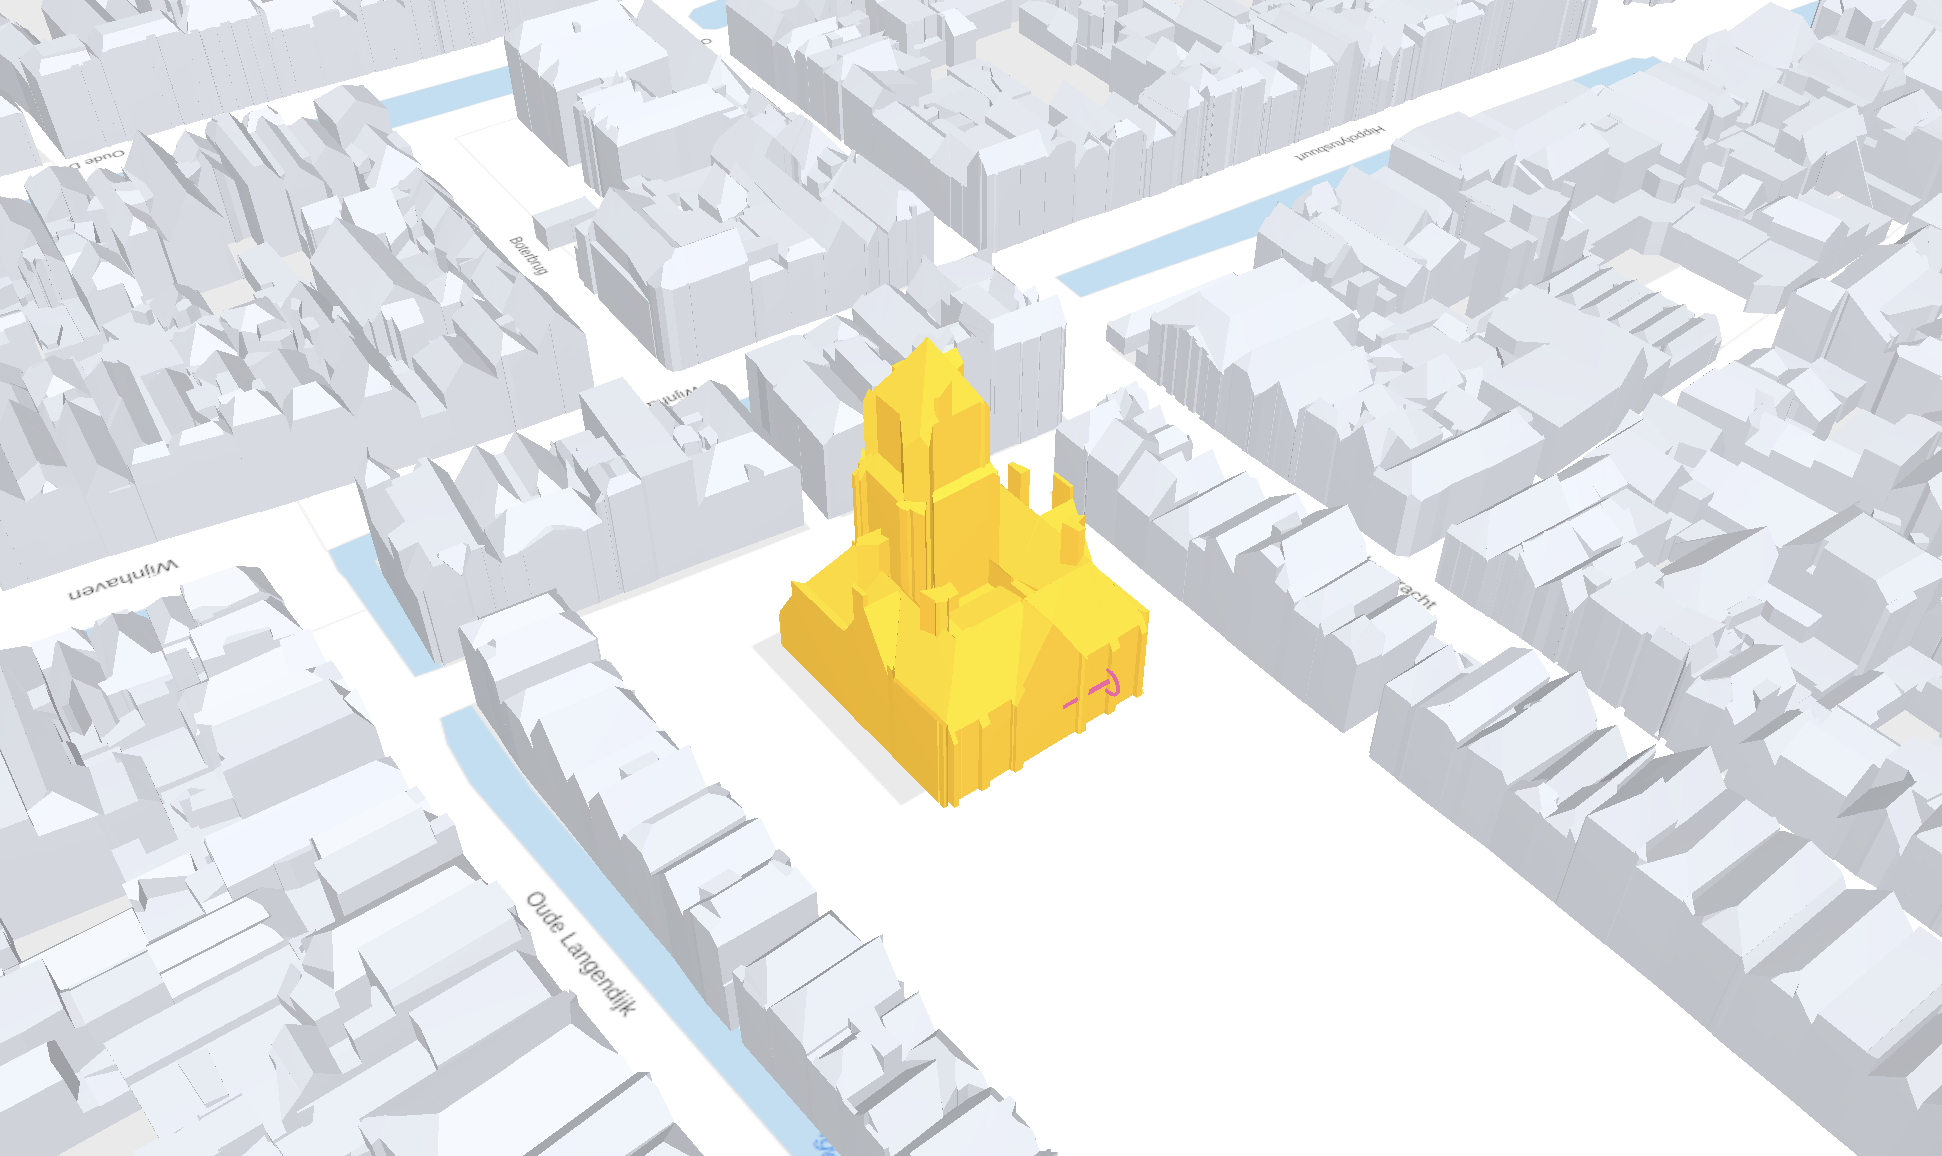
\includegraphics[width=\linewidth]{figures/3dbag.png}
\caption{A small part of the 3DBAG\protect\footnotemark 3D city model of the Netherlands with a building highlighted}
\label{fig:3dbag}
\end{figure}
\footnotetext{\url{https://3dbag.nl/en/viewer}}

% How 3D city models are created
3D city models can be created using largely manual methods involving modelling individual buildings, but such methods are expensive and cannot be scaled to large areas.
Instead, we are interested in the (semi-)automated creation of 3D city models, and the most common automated approach involves merging two datasets: (1) a 2D topographic dataset containing polygons for the features that will be represented and (2) an elevation dataset that is used to process the 2D geometries and lift them to 3D.
For example, the former dataset could contain individual polygons that represent building footprints, while the latter could consist of a point cloud that is used to obtain the height of the buildings' roofs.
Alternative approaches exist, such as first obtaining a dense mesh (e.g. through dense matching of images) that is then classified or more recently the automated conversion from BIM-to-Geo, but these typically require data that is more expensive to acquire and more complex to process.

While the aforementioned method with two datasets (topography + elevation) is relatively simple to apply in practice, these two datasets are not available in many countries, or at least not available openly, in a suitable form and at a sufficient quality for the creation of a 3D city model.
As a result, 3D city models are only openly available for a limited number of cities in around 20 countries\footnote{\url{https://3d.bk.tudelft.nl/opendata/opencities/}}, which are situated almost entirely within the Global North---where topographic data is generally more widely available and elevation data tends to have higher resolution.

% Issues with Mexico specifically
In the case of Mexico, while both topography and elevation are available for the entire country, there are significant issues with respect to the available features, coverage and resolution of these datasets (Section \ref{sec:data}).
Most importantly, the objects that are considered the most important features in 3D city models (buildings and roads) are not individually modelled in the 2D topography, whereas the coverage of high-resolution 1.5-metre elevation models is limited to a few areas around some of the bigger cities.
Likely as a result, to the best of our knowledge, no 3D city models are openly available for any city in Mexico, and academic efforts to create them are limited to small areas using custom data, and either largely manual modelling methods or closed solutions with commercial closed source software  \citep{HernandezSanchez20,RiveraGonzalez2020,GaliciaReyes22}.

Nevertheless, in this paper we aim to show that it is possible to create 3D city models automatically for the areas in Mexico where high-resolution elevation data is available based solely on open data (elevation + 2D topography).
For this, we propose a novel methodology (Section \ref{sec:methodology}) that is partly inspired by earlier implementations (see Section \ref{sec:implementation} for the details), but specifically targets the particularities of the source data.
The methodology extracts building footprints from the elevation data and roads from the empty spaces between city blocks.
These are complemented with existing areal features for green areas, water bodies and city blocks.
Finally, the resulting polygons are lifted using three different rules (flat to a percentile height, vertices to a generated TIN, and vertices + interior points to the TIN), which are customisable and automatically set the heights according to statistical measures that are computed with the available elevation data sets (a DTM and a DSM).

This methodology has been implemented (Section \ref{sec:implementation}) and tested in an area of central Mexico City that combines a mix of varied buildings from detached homes to skyscrapers and incorporates a variety of land uses (including green areas and water bodies) and significantly changing elevations.
Preliminary results (Section \ref{sec:results}) show that while not all buildings can be detected, the newly created building footprints are often more accurate than those available in the open footprint data sets from Microsoft and Google.
Also, unlike the latter datasets, our methodology is able to create non-rectilinear building footprints.
Since these buildings are frequently city landmarks, it results in 3D city models that are also clearly distinguishable.

% Within the abstract and the subsequent full paper, we have the following related objectives: (1) to describe the most promising open datasets that are currently available for the creation of 3D city models in Mexico, (2) to discuss the issues in them that make it challenging to use the data for this purpose, (3) to propose a methodology that can be used to overcome some of the data issues, and (4) to test the methodology and create 3D city models of some areas.

\section{Available datasets, their characteristics and their issues}
\label{sec:data}

As mentioned in the introduction, both 2D topographic datasets and an elevation datasets are available in Mexico.
However, there are significant issues with respect to their available features, coverage and resolution.

\subsection{2D topography}

At the national level, the National Institute of Statistics and Geography (INEGI)\footnote{\url{https://www.inegi.org.mx}} provides different relevant datasets related to topography.
Among these, the likely best source is the 1:50 000 vector topographic dataset (Figure \ref{fig:50k}), which contains several useful polygonal datasets, including some land use types (e.g. school, recreational/sport, public area, railway station), water-related features (e.g. water bodies, canals and ponds) and city blocks (i.e.\ a buildable area that is usually surrounded by roads)---a fundamental unit of urban structure known as \emph{manzana} in Spanish.
However, roads and railways are only represented as centre lines and building footprints are not available, which means that the most important classes for a 3D city model are missing in areal form.

\begin{figure}[htbp]
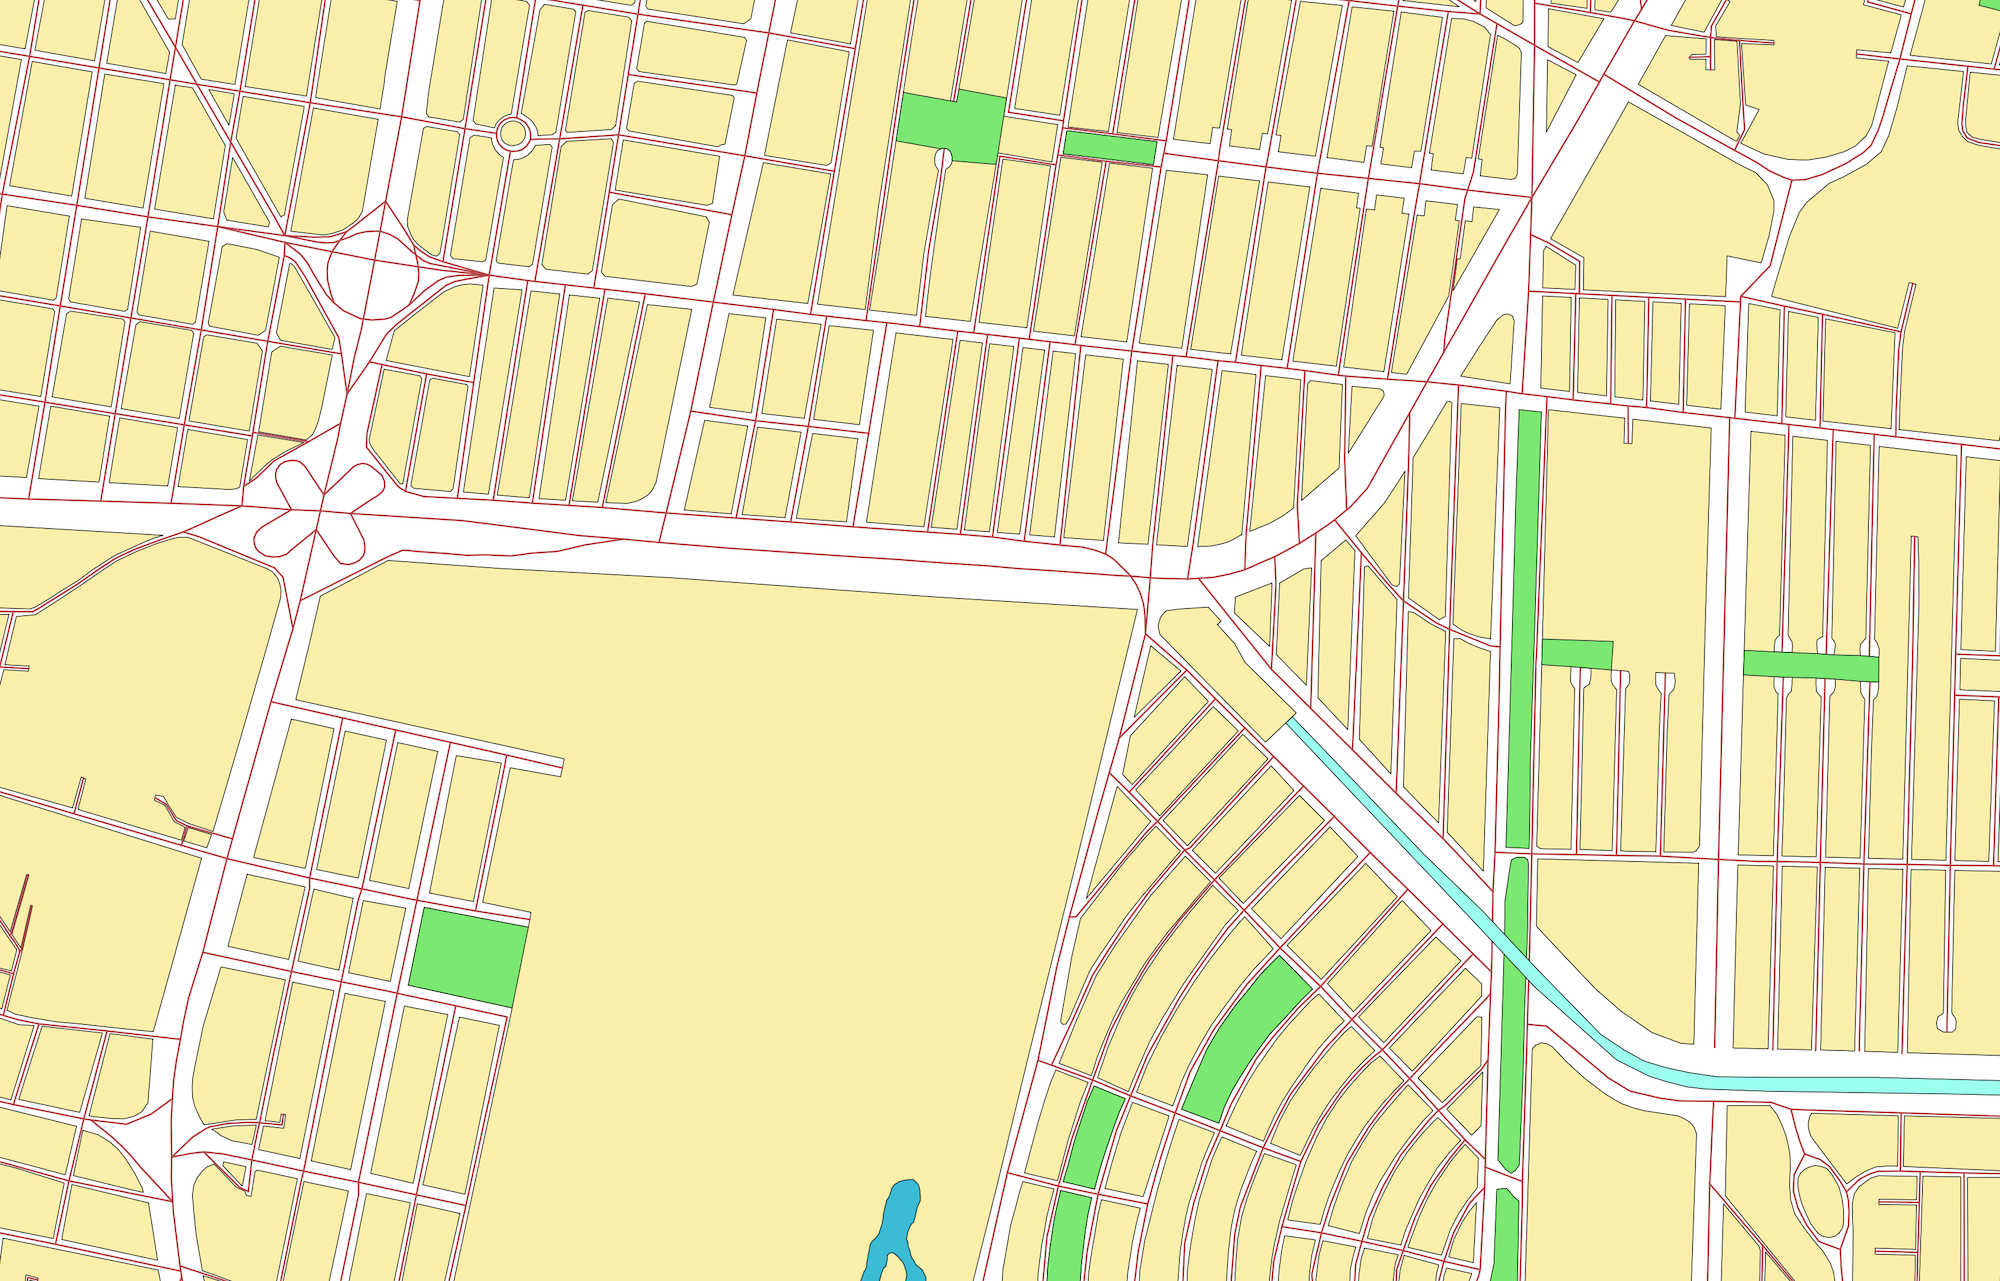
\includegraphics[width=\linewidth]{figures/50k.png}
\caption{Some of the topographic features available in the 1:50 000 vector topographic dataset from INEGI: city blocks (yellow), roads (red lines), public areas (green), water bodies and canals (blue).}
\label{fig:50k}
\end{figure}

Since cadastral data in Mexico is managed at the state level and the built area of the buildings in each plot is often used for the calculation of property taxes, it could be expected that building footprints would be available from local governments.
However, even in the cases where building footprints are clearly recorded (Figure \ref{fig:angel}), they are not publicly available for download.

\begin{figure}[htbp]
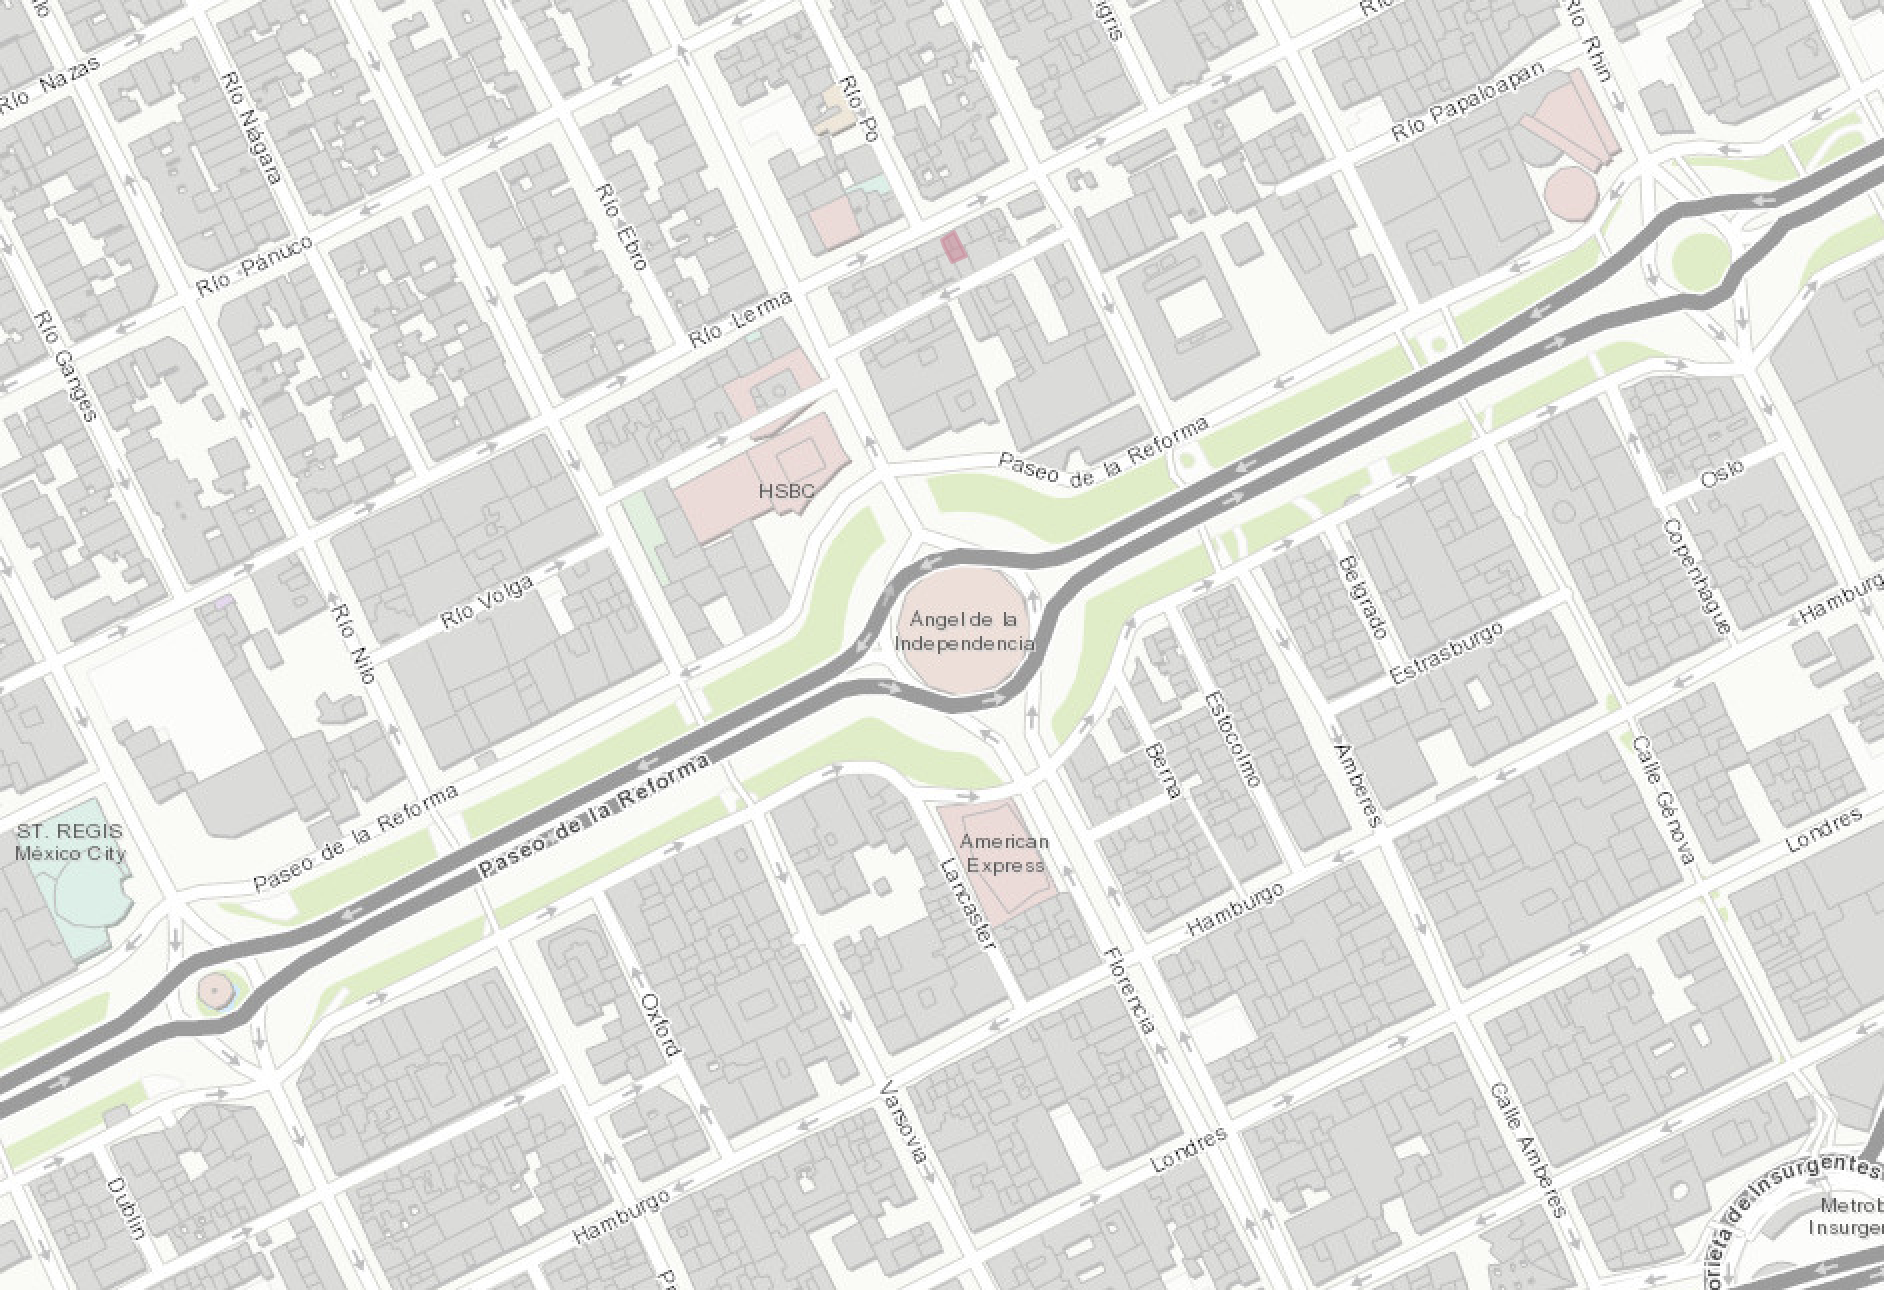
\includegraphics[width=\linewidth]{figures/angel.png}
\caption{Building footprints are visible in the Mexico City Open GIS\protect\footnotemark but they are not available for download.}
\label{fig:angel}
\end{figure}
\footnotetext{\url{https://sig.cdmx.gob.mx/sig_cdmx/}}

Alternatively, in the specific case of building footprints, it is possible to obtain them from some global datasets, such as the Mi\-cro\-soft Glo\-bal\-ML\-Buil\-ding\-Foot\-prints dataset\footnote{\url{https://github.com/microsoft/GlobalMLBuildingFootprints/}}, which covers part of Mexico, or Google's Open Buildings dataset\footnote{\url{https://sites.research.google/gr/open-buildings/}} \citep{Sirko21}, which covers all of Mexico (Figure \ref{fig:footprints}).
However, our initial tests show that these building footprints are quite accurate for isolated buildings in more rural or suburban settings, but they do not fit real-world buildings well when buildings are closely-spaced in denser urban areas.

\begin{figure}[htbp]
\begin{subfigure}{\linewidth}
    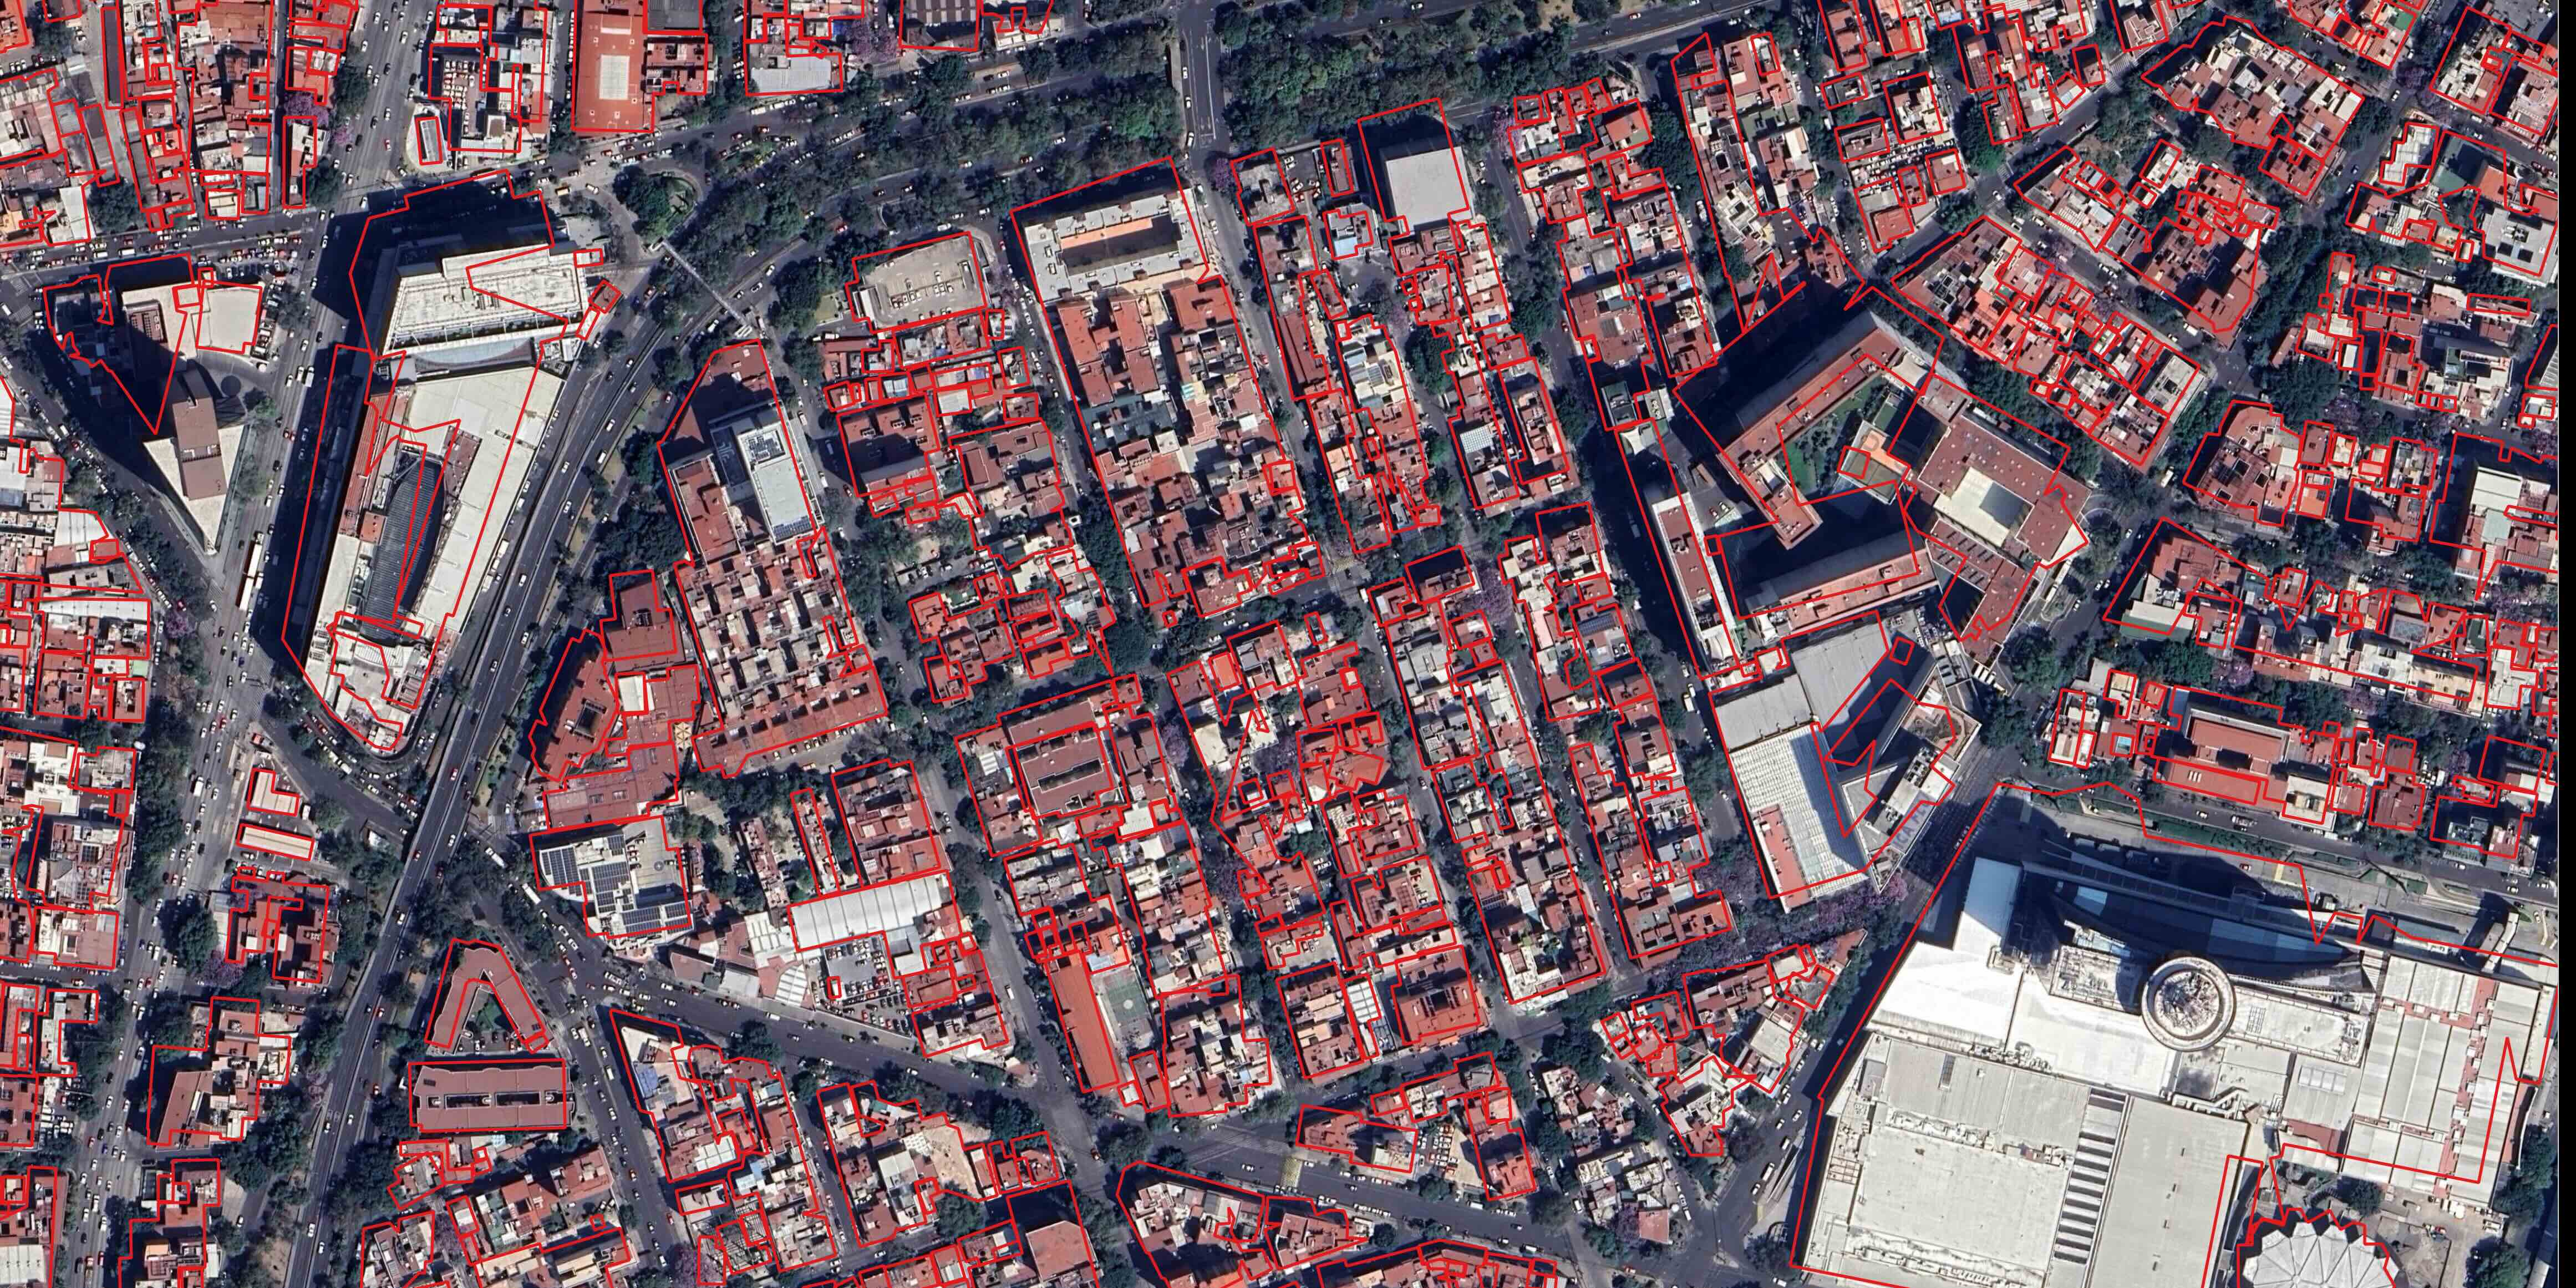
\includegraphics[width=\linewidth]{figures/footprints-ms.jpg}
    \caption{}
    \label{fig:footprints-ms}
\end{subfigure}
\begin{subfigure}{\linewidth}
    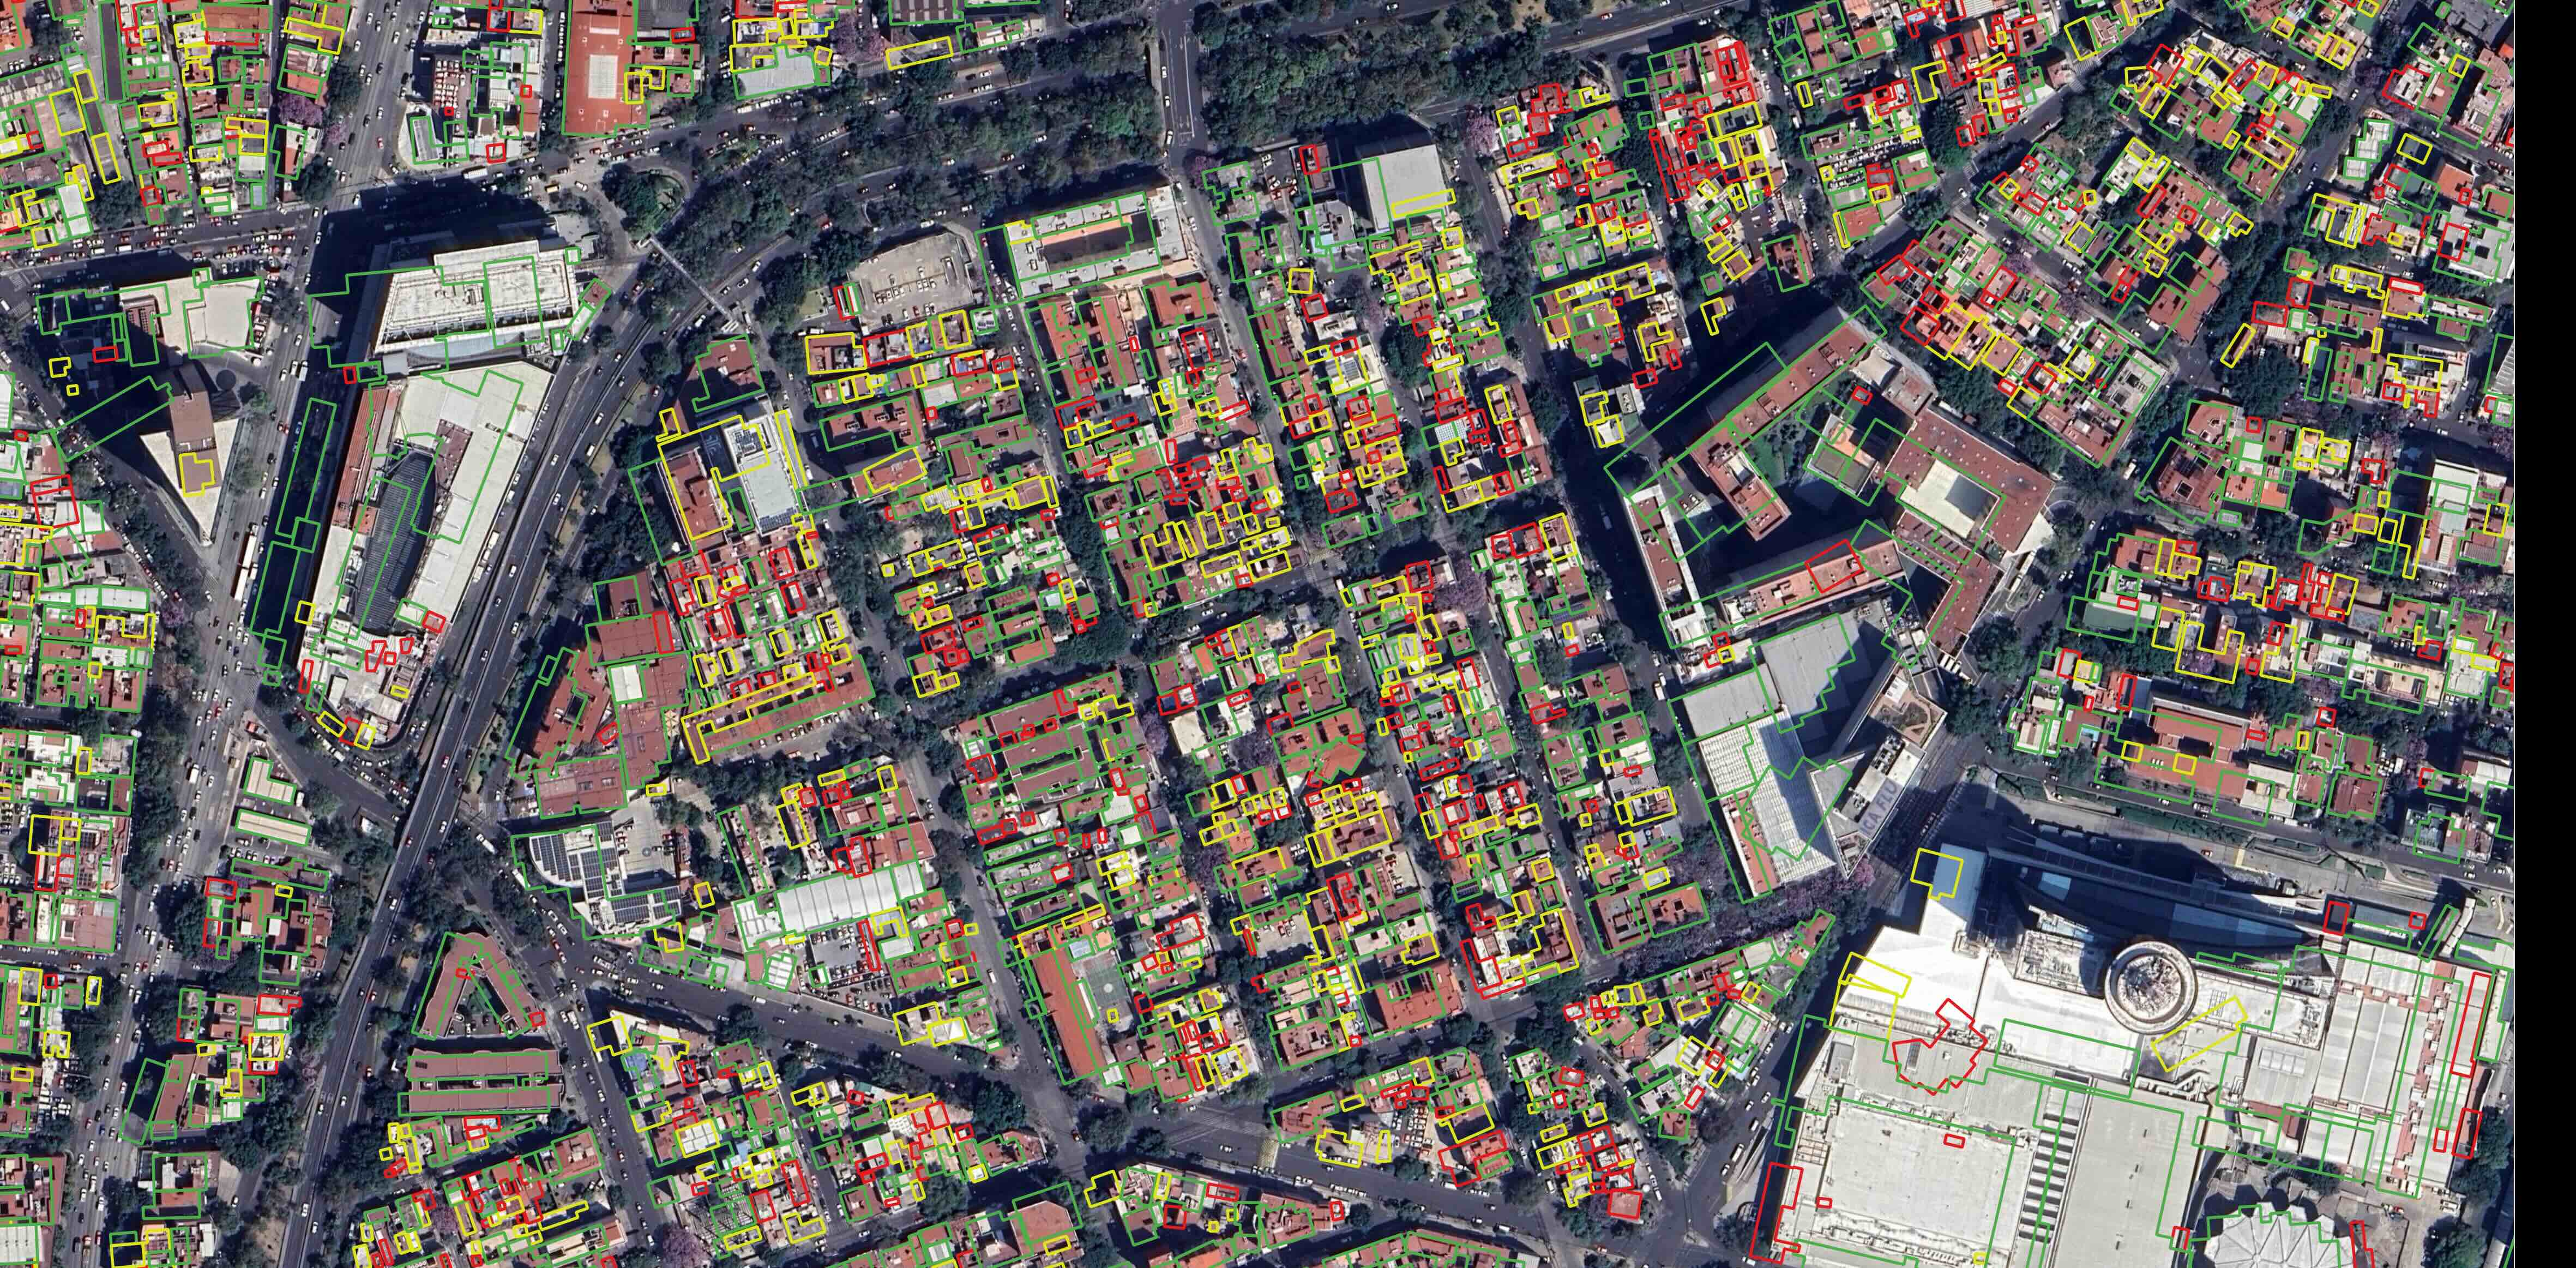
\includegraphics[width=\linewidth]{figures/footprints-google.jpg}
    \caption{}
    \label{fig:footprints-google}
\end{subfigure}
\begin{subfigure}{\linewidth}
    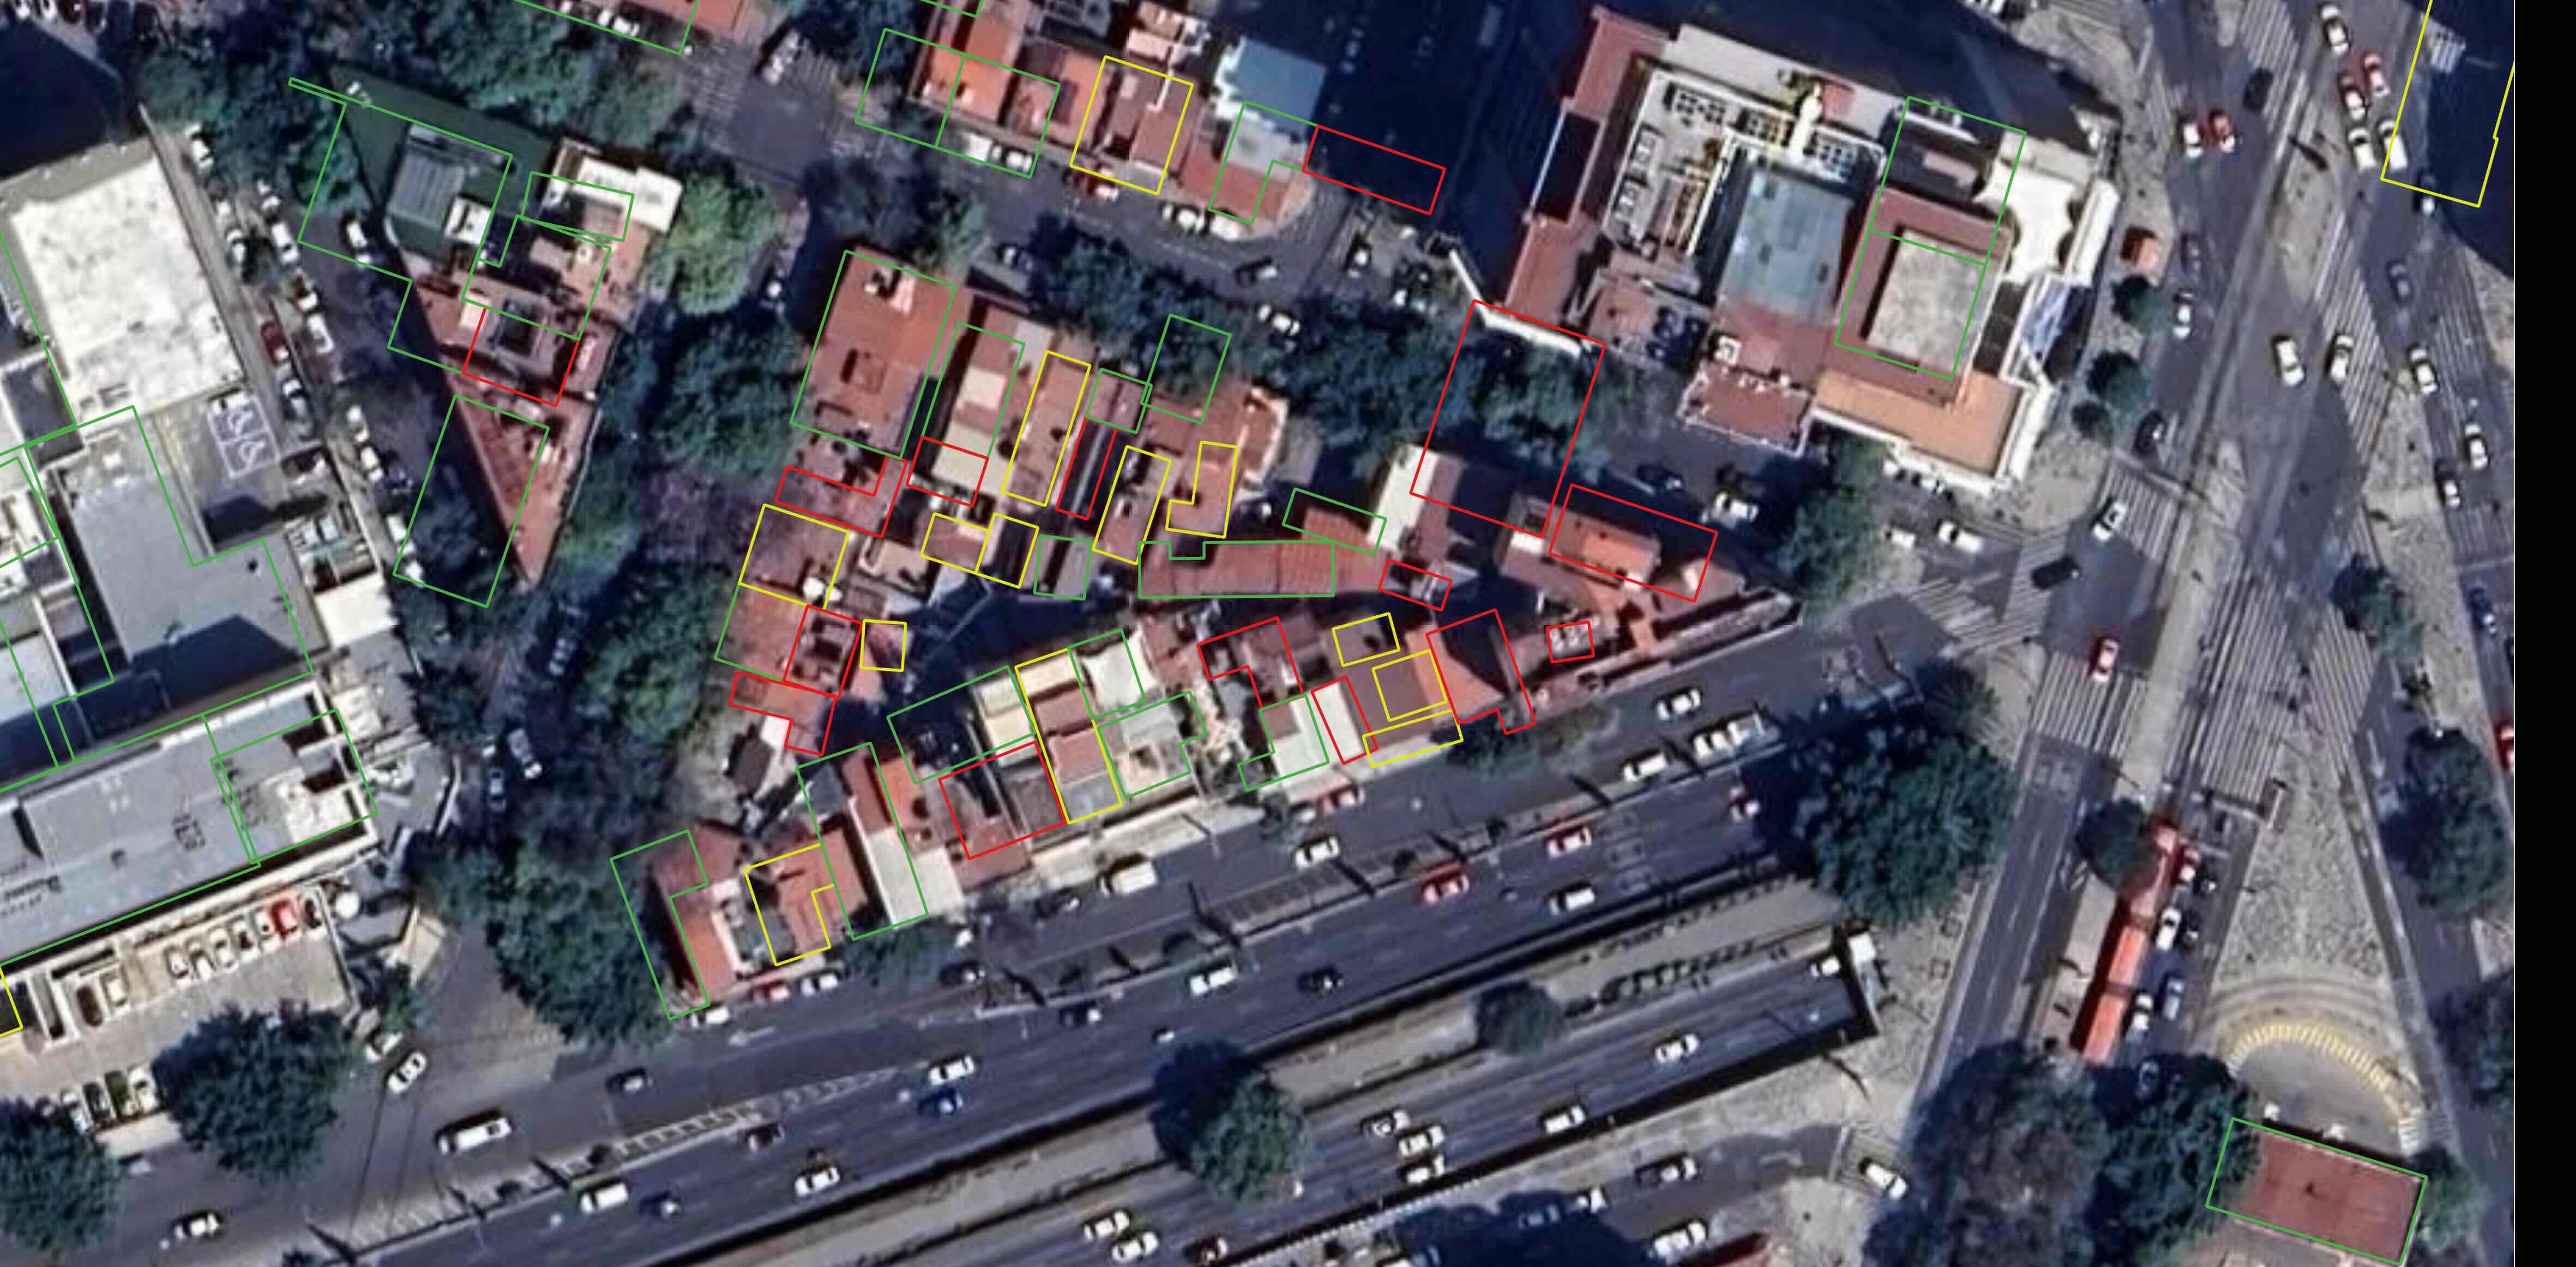
\includegraphics[width=\linewidth]{figures/footprints-google-zoom.jpg}
    \caption{}
    \label{fig:footprints-google-zoom}
\end{subfigure}
\caption{(a) The Microsoft building footprints dataset systematically undersegments dense built-up areas, often resulting in entire blocks merged into one polygon. (b) Google seems to do better at capturing more buildings, but (c) it actually oversegments the data, creating new polygons for smaller rooftop features and for clearly non-existing buildings. The colours in Google's data represent the confidence value stored in the dataset (green $>$ 0.75, 0.75 $>$ yellow $>$ 0.7, 0.7 $>$ red). Note that both datasets have spurious buildings, including in roads, and do not support non-rectilinear buildings.}
\label{fig:footprints}
\end{figure}

Finally, an interesting alternative for the Mexican case is to take advantage of the high-resolution elevation data that is openly available from INEGI for some areas in Mexico (see the following section), which can be used to extract buildings by assuming that these have significantly different roof heights or a separation of at least one pixel (i.e. 1.5 metres if high-resolution data is available).

\subsection{Elevation}

INEGI also provides various elevation datasets, including a nationwide digital terrain model (DTM) with 15-metre resolution, as well as higher resolution DTMs and digital surface models (DSMs) that are available in certain parts of the country\footnote{\url{https://www.arcgis.com/apps/mapviewer/index.html?webmap=b593168ba9784bbc9dd4b909407e559a}}.
In the context of 3D city models, the latter datasets are the most interesting, since these are the models in which the elevation of building roofs, road surfaces and the top of other features (e.g. tree canopies) can be distinguished---at least when these do not overlap each other.
However, it is worth noting that while it is not tested in this article, the lower-resolution 15-metre dataset should still be usable to generate country-wide 3D geometries for most features with the notable exception of buildings.

The high-resolution DSMs from INEGI are all raster models but come in different forms: mostly older 5-metre resolution models with wider coverage (about a third of the country), newer 1.5-metre models only in and around some bigger cities, and a mix of other models derived from specific projects (e.g. 2.5-metre data in the Tren Maya region).
These datasets are acquired through a mix of methods: photogrammetry from satellite and aerial imagery as well as LiDAR surveys.
Buildings that are wider than the resolution of these datasets can usually be seen in these DSMs (Figure \ref{fig:altura}), but artefacts are sometimes present (e.g. the sides of tall buildings being visible) and the features in the DSMs are not always sharp, particularly when the data is generated from satellite imagery.

\begin{figure}[htbp]
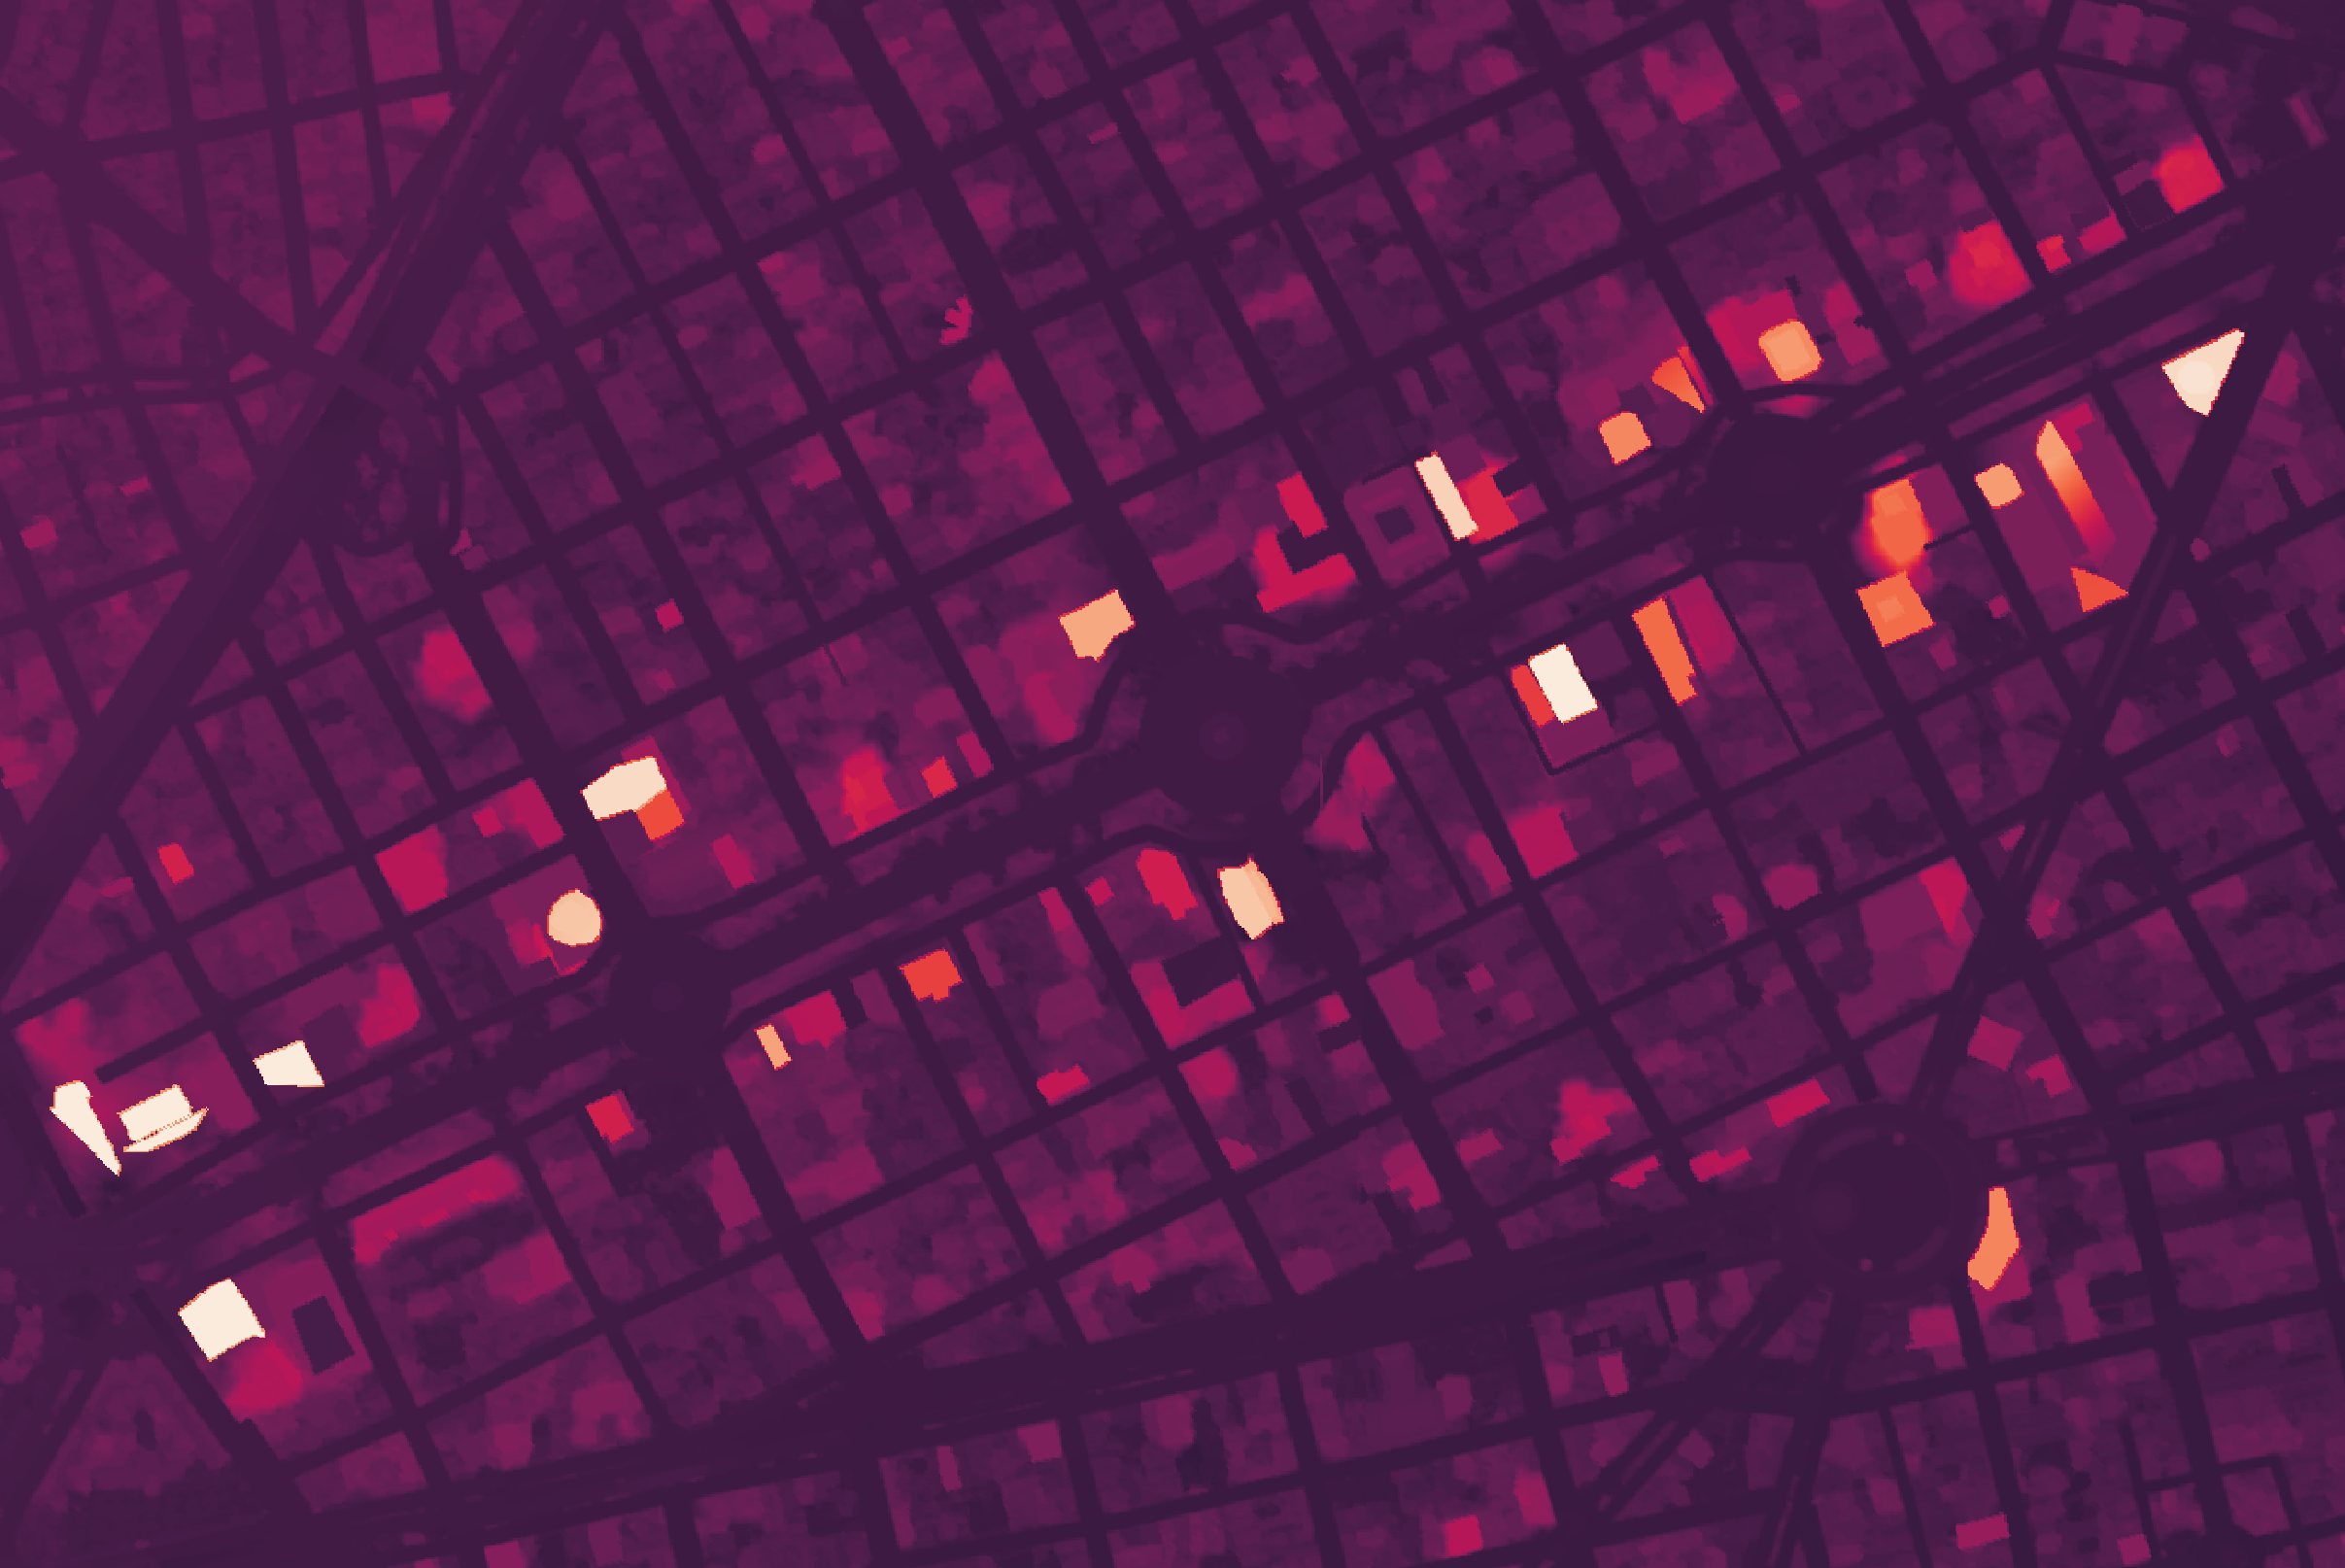
\includegraphics[width=\linewidth]{figures/altura.png}
\caption{Individual buildings can be clearly seen in the 1.5-meter DSM from INEGI}
\label{fig:altura}
\end{figure}

In addition to the INEGI data, there are other datasets that could be used for the elevation information, e.g. the ALOS Global Digital Surface Model\footnote{\url{https://www.eorc.jaxa.jp/ALOS/en/dataset/aw3d30/aw3d30_e.htm}} \citep{Takaku14} at 30-meter resolution.
However, we are not aware of any other open datasets that are available in Mexico and which have a higher resolution than the INEGI data.

\section{Methodology}
\label{sec:methodology}

% In the full paper, we will include a more thorough evaluation of the datasets from Section \ref{sec:data} for the creation of 3D city models, describe a few methods that can be used to create polygons for the main missing features (i.e. buildings and roads), as well as to lift these polygons to the appropriate height, show our implementation and the results of the creation of some 3D city models---partly based on the methodology of \citet{3dfier}---and evaluate the quality of the 3D city models that could be produced.

\subsection{Generation of road, railway and water stream polygons}

We first compute a Boolean set union of some of the areal types present in the 1:50 000 vector topographic dataset from INEGI.
Mainly, this includes city blocks, but also other types which are not always covered by the city blocks, including the land use and water-related features mentioned previously.
After this process, most of the areas not covered are roads, with the remainder being railways (apart from station areas) and smaller water streams.
These remaining areas can therefore be extracted as a Boolean set complement, or alternatively by subtracting individual areal types from a particular study area (e.g.\ a tile of the INEGI data).

Finally, since these roads, railways and water streams (\emph{corrientes de agua}) are modelled as lines in the INEGI data, the remaining areas can be classified by proximity to these lines, which also makes it possible to assign the semantics present in the linear data to the newly created areas.
Alternatively, as a first approximation which is accurate in many areas, it is also possible to simply consider all the areas left as roads.

\subsection{Generation of building footprint polygons}

The first step is to subtract the DTM from the DSM, resulting in a map that contains only the height of the objects in it.
Then, we use the newly computed polygons from the previous step (roads, railways and water streams), as well as the feature types from the INEGI data where buildings should not be present (e.g. green areas and water bodies) to mark all these areas with the NODATA value of the raster.
This is done to avoid generating buildings in these areas, since it is sometimes difficult to distinguish buildings from tree canopies.

Next, we use a region-growing-like algorithm that starts from seed points in this raster and grows them to complete building footprints.
For this, we use all points in the raster with a height of at least 10 metres.
This parameter is set somewhat arbitrarily at a value where we consider that points are more likely to represent building roofs than tree canopies.
However, this parameter should be fine-tuned based on the vegetation and building heights in the study area.
Higher values will generate fewer incorrect footprints from tall vegetation but will also miss shorter buildings, whereas lower values will include more building footprints but also more false footprints from vegetation.

Starting from these points, the growing condition considers that pixels are 4-connected and has two height difference tolerance thresholds to stop the region growth.
For buildings taller than 100 meters, a height difference between neighbouring pixels of 15 metres is allowed in order to capture steeply inclined fa\c{c}ades and building spires.
Since such high-rise buildings are always separated by a few pixels, such a high threshold is not a problem and does not result in merged buildings.
For shorter buildings, which often have no discernible separation between them, the height difference is reduced to 0.75 metres (equivalent to a 1/2 gradient) in order to avoid merging adjacent buildings whenever possible.

In order to get rid of spurious buildings and artefacts in the original data, we only keep the polygons with an area of at least 45 pixels (about 100 m$^2$).
The outlines of these buildings are generated (polygonised), and are then simplified using the Visvalingam–Whyatt algorithm \citep{Visvalingam93} with a tolerance of 3 meters (i.e. 2 pixels), which removes the staircase effect caused by the raster input.
A sample of the resulting building footprints generated can be seen in Figure \ref{fig:footprints-this}.

\begin{figure}[htbp]
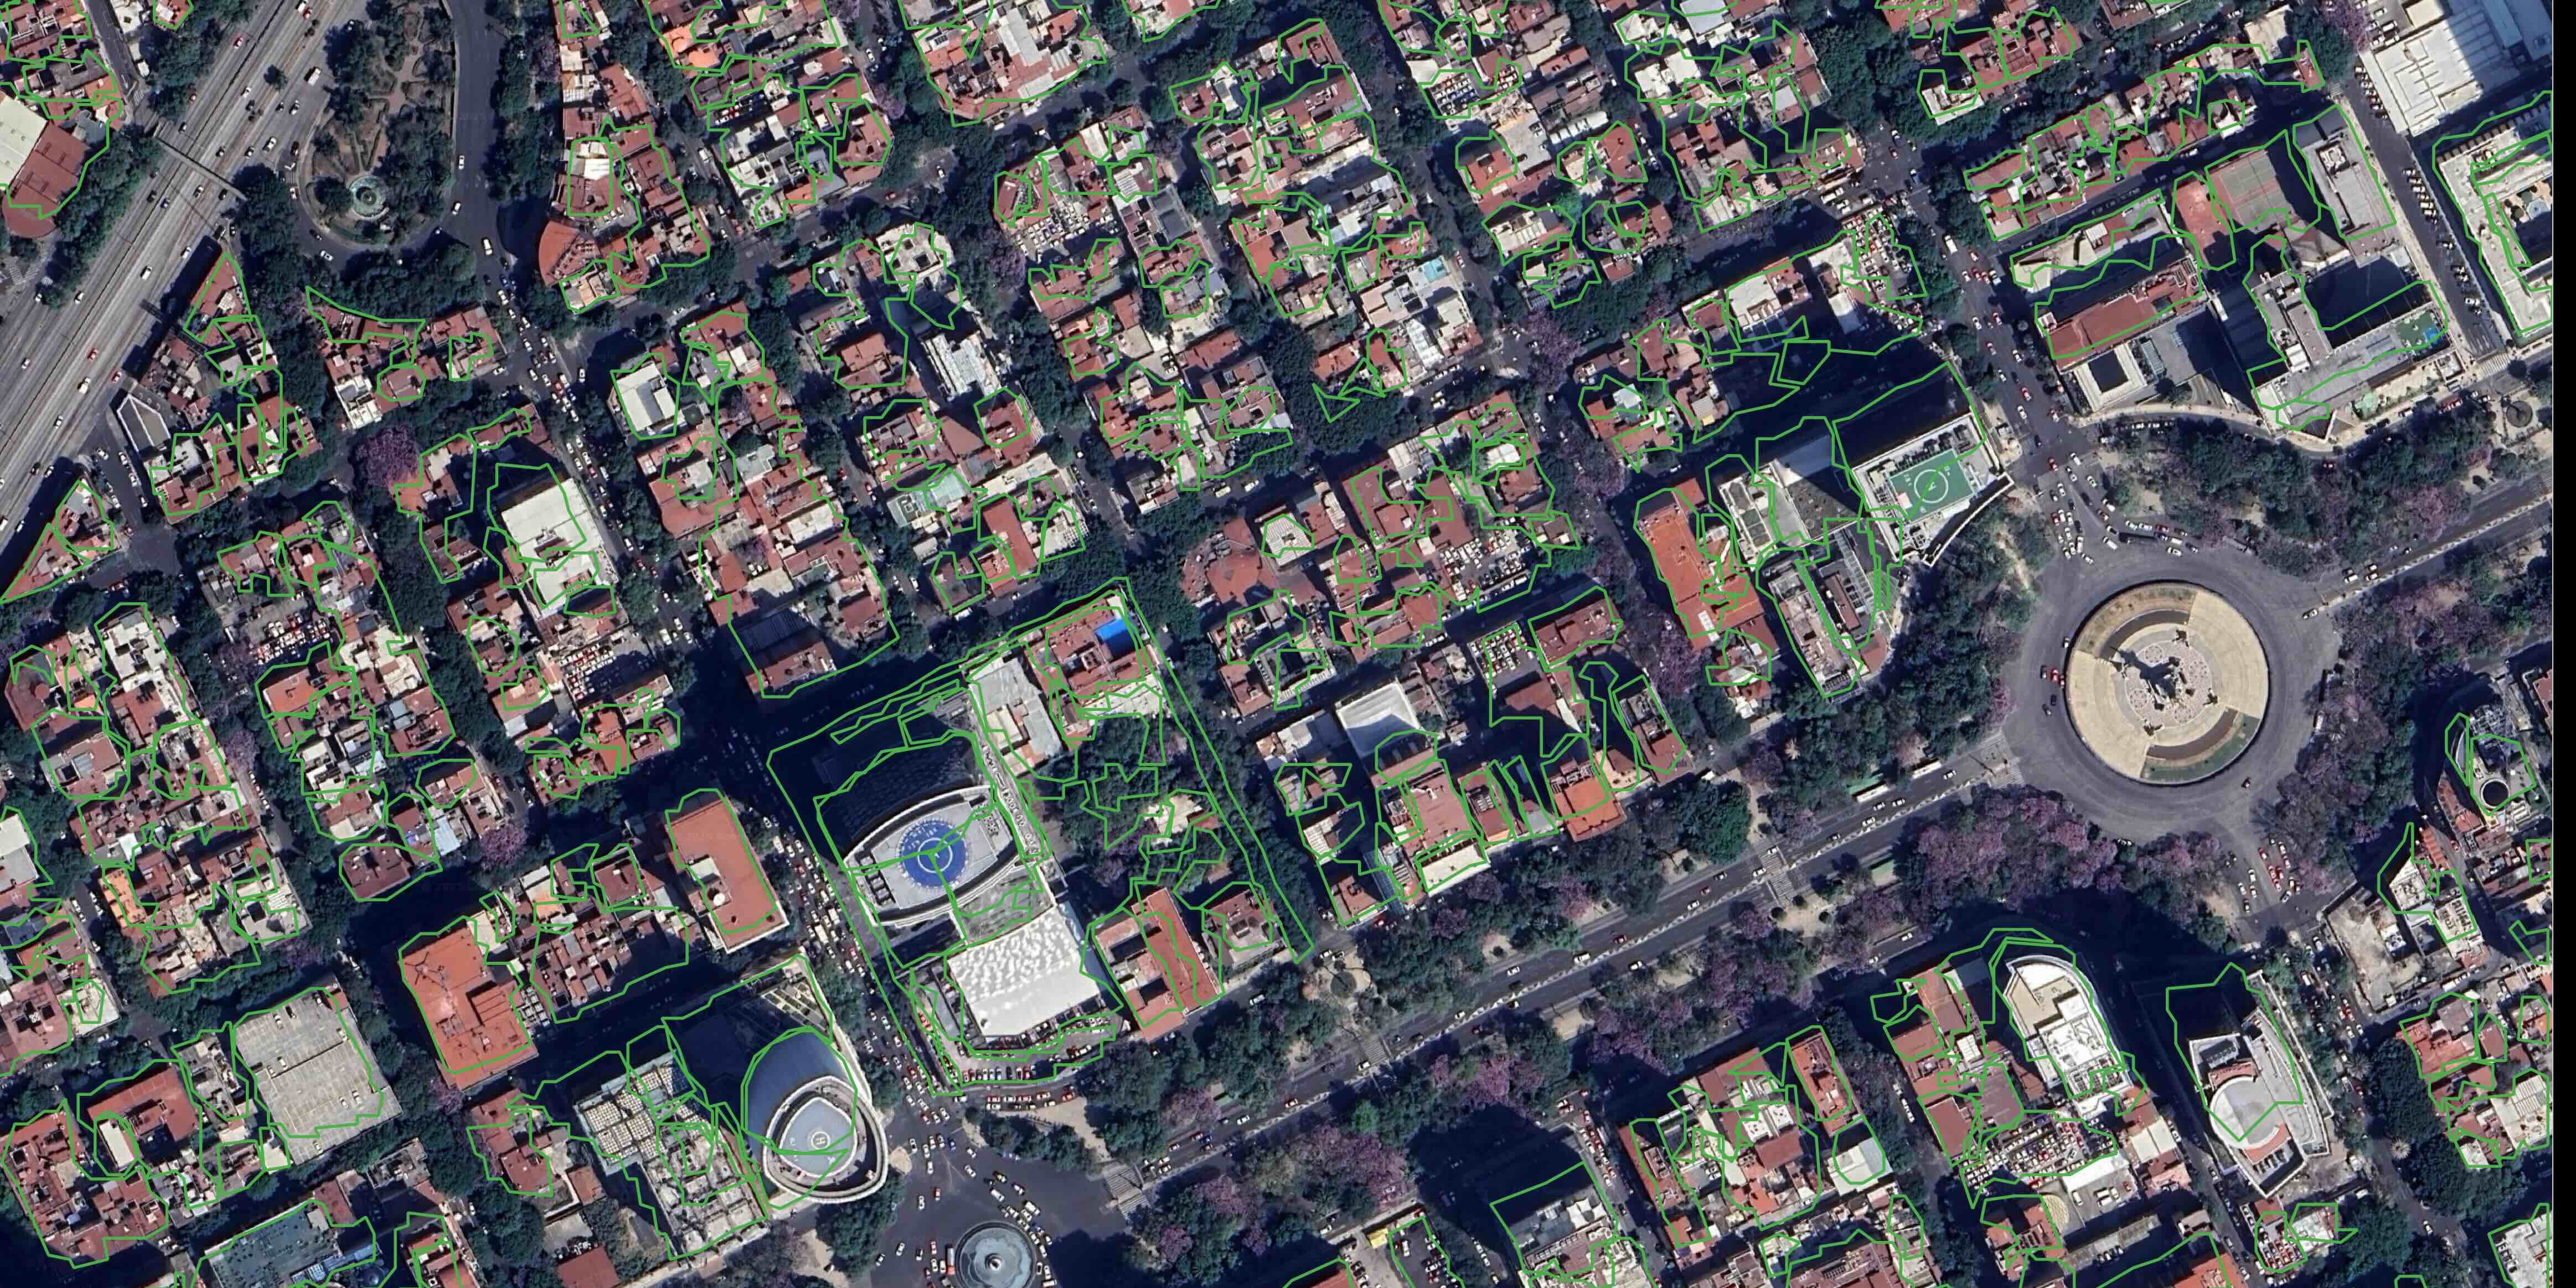
\includegraphics[width=\linewidth]{figures/footprints-this.jpg}
\caption{The building footprints that were created using the INEGI data. By taking advantage of the DSM data and not enforcing strict rectilinear polygons, the method creates reasonably accurate building footprints for complex buildings.}
\label{fig:footprints-this}
\end{figure}

\subsection{Data preprocessing}

To prepare the data for lifting, we apply two main preprocessing steps.
For the vector data, all polygons are repaired and triangulated using the method in \citet{Ledoux14}, which is available in the CGAL Polygon repair package\footnote{\url{https://doc.cgal.org/latest/Polygon_repair/index.html}}.
In brief, it consists of a constrained Delaunay triangulation of the polygon's edges, which is then followed by a labelling of exterior/interior triangles using an odd-even counting mechanism. 
The triangles that are marked as interior are those that are part of the polygon and will be used for subsequent processing.

Since the elevation models' resolution is relatively high, we also create a simplified DTM stored as a TIN using points every 30 metres on a grid.
For each point along the 30-metre grid, the DTM points within 120 meters are obtained and the elevation of the point is set to their average.
This TIN can be used to add details to certain feature types (e.g. vegetation height in plant cover areas) without significantly increasing the size of the model.

\subsection{Polygon lifting}

For the polygon lifting, we start from the road and building footprint polygons generated in the previous steps, as well as other polygons directly obtained from the INEGI data (plant cover from public areas, water bodies and terrain from city blocks).
These are shown in Figure \ref{fig:polygons}.

\begin{figure}[htbp]
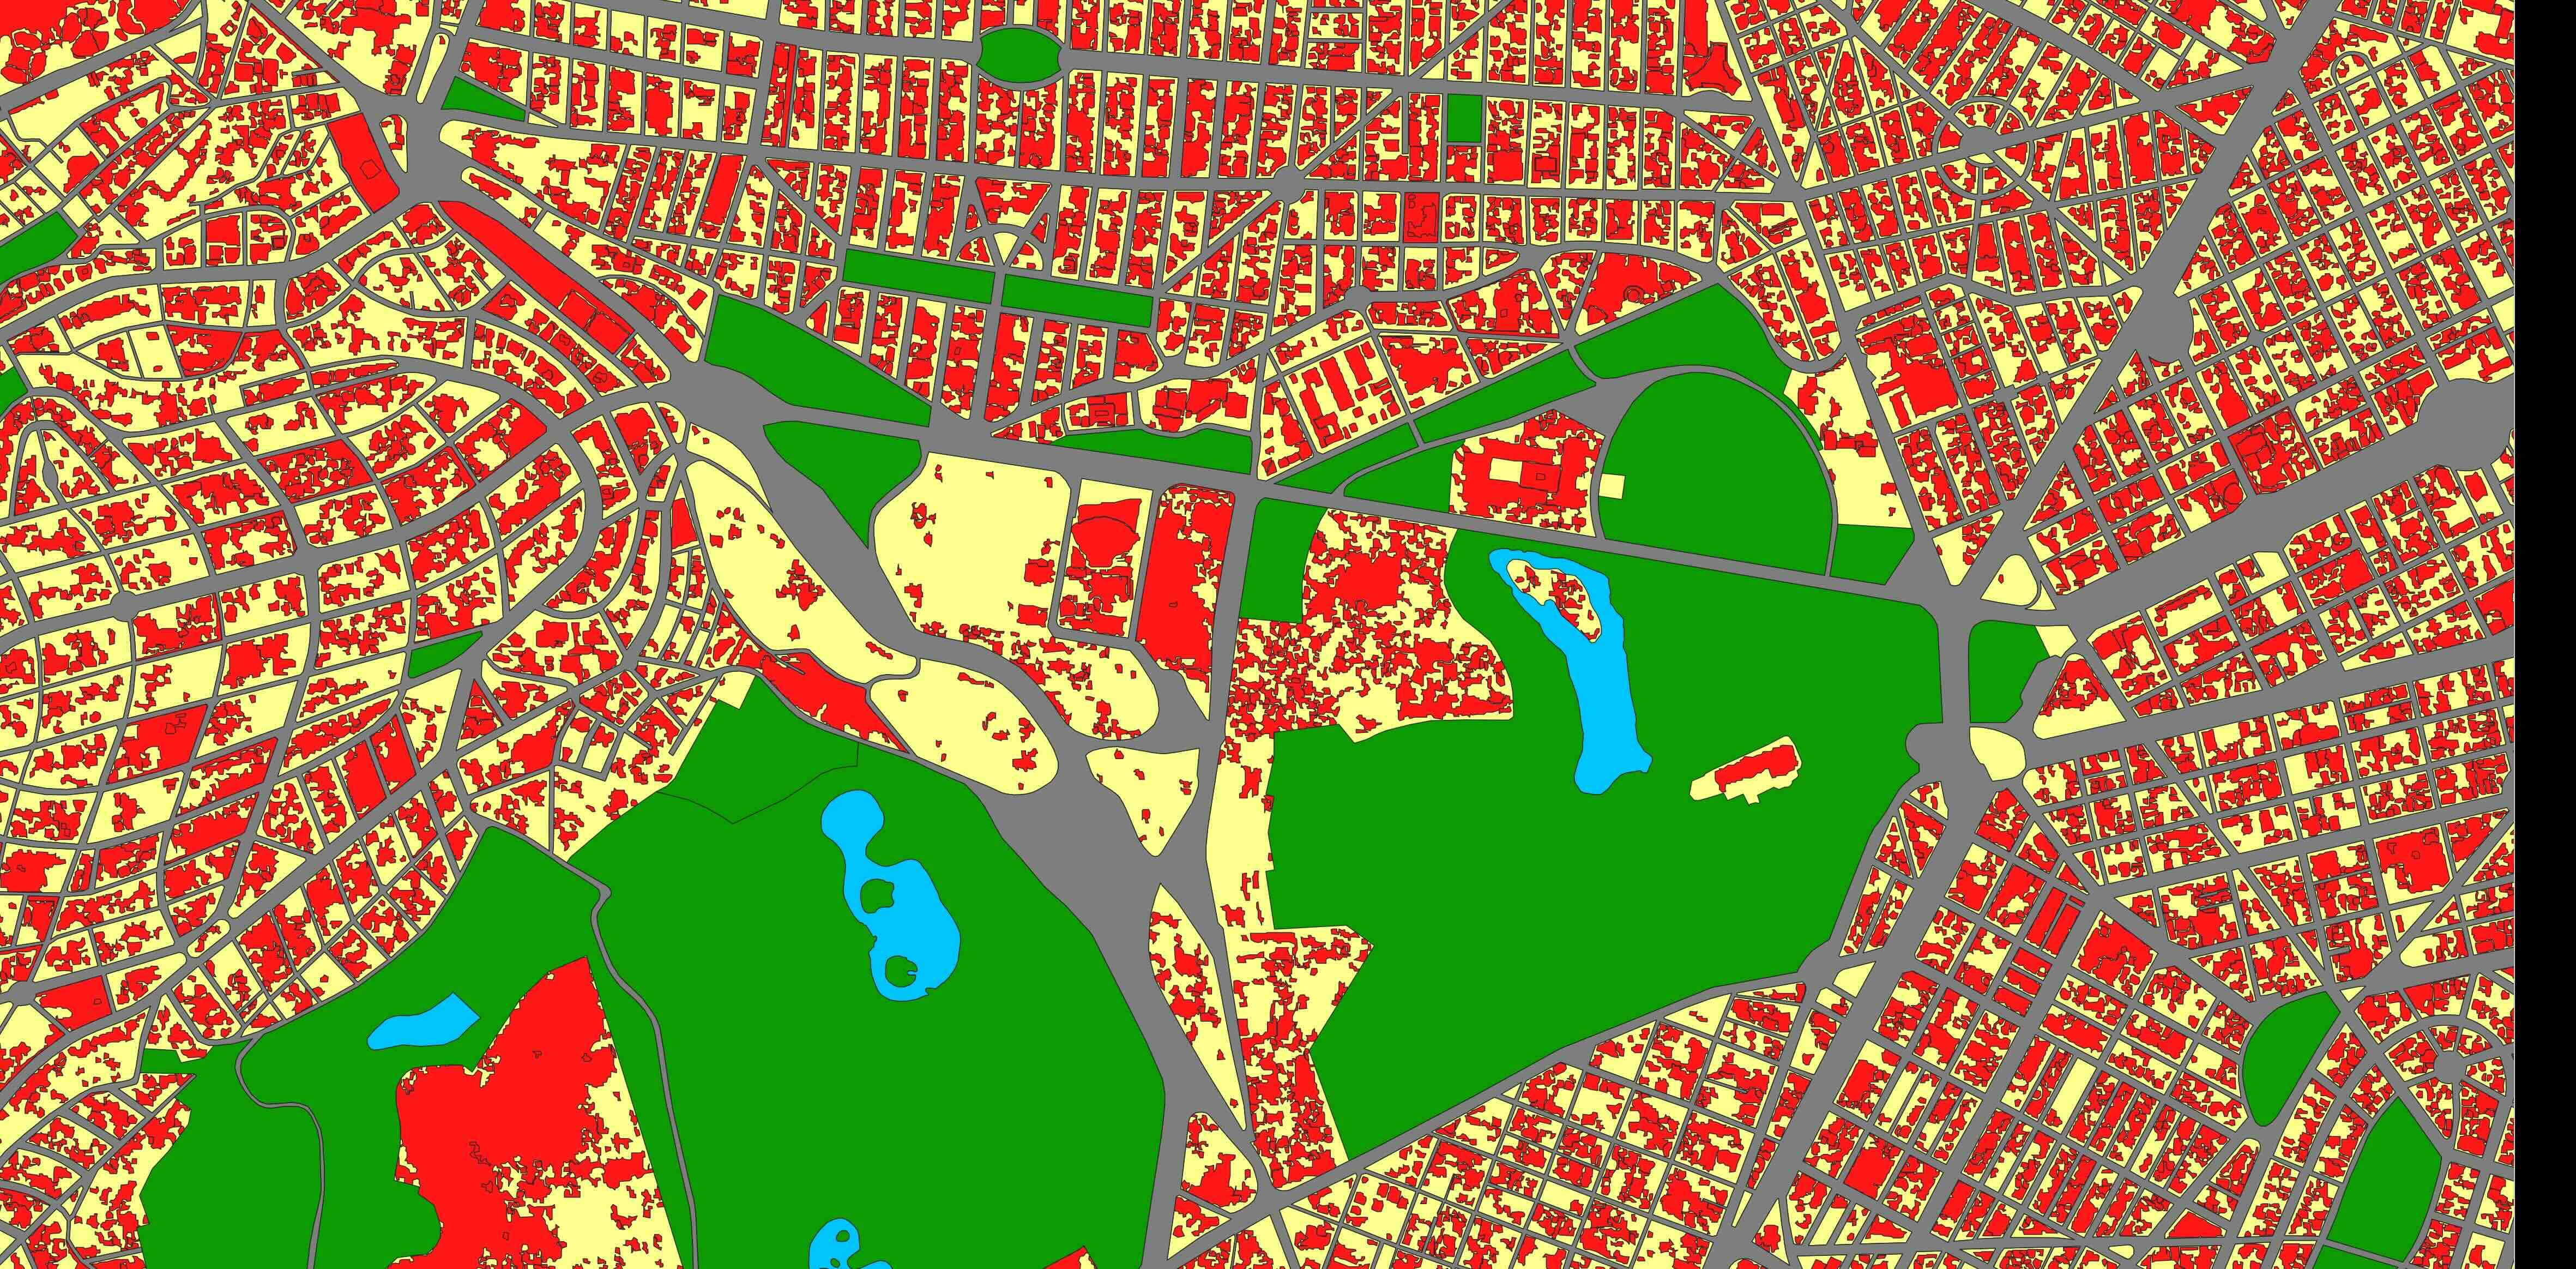
\includegraphics[width=\linewidth]{figures/polygons.jpg}
\caption{The polygons that are lifted: roads, building footprints, plant cover, water bodies and terrain.}
\label{fig:polygons}
\end{figure}

These polygons are lifted according to three rules:

\begin{description}
    \item[Flat polygon lifting] Each building footprint is lifted uniformly to the same height, which is computed as the 90th percentile value of all the DSM points that are inside the polygon. This is done to obtain something close to the maximum height of a building but avoiding outliers in the DSM data.
    \item[Vertices lifting] The vertices of the road, water body and terrain polygons are lifted to their level in the DTM TIN.
    \item[Vertices lifting with additional points] The vertices of the plant cover polygons are lifted to their level in the DTM TIN, and the TIN points that fall inside the polygons are also added. This involves retriangulating the interior of the polygon using a constrained Delaunay triangulation in a 2D $XY$ projection of the polygon.
\end{description}

After the polygons are lifted, vertical surfaces are generated to close the gaps between the differently lifted polygons.
In practice, this is mostly for the buildings' walls, but it could also be done to other feature types when these are lifted to a flat height.
For instance, this could be done with water bodies (to a low percentile value).

\subsection{CityJSON and OBJ output}

Finally, the lifted polygons are written as a 3D city model in two forms:

\begin{itemize}
    \item Wavefront OBJ models for easy visualisation in any 3D graphics software, or alternatively in the built-in viewers available in both Windows and macOS. The simplified DTM can also be written in this way for debugging or parameter optimisation purposes. A material definition file is used to provide intuitive colours for the different feature types.
    \item CityJSON \citep{Ledoux19} models with the semantics for each object, which are mapped to the Building, Road, PlantCover and WaterBody classes. The buildings correspond to LoD1 in the CityGML data model \citep{citygml2021ogc} and also have semantic surfaces (RoofSurface, WallSurface and GroundSurface). 
\end{itemize}

\section{Implementation}
\label{sec:implementation}

The methodology was implemented with a variety of scripts in Python and C++, as well as using existing functionality in QGIS.
The scripts that were developed have been made available at \url{https://github.com/kenohori/3dcm-mexico}.
In particular:

\begin{itemize}
    \item The Python script \texttt{buildinggrower.py} implements the region-growing algorithm starting from the DSM-DTM grid where the classes in which buildings are not expected are set to NODATA (or to a very low value). Raster input/output is implemented with Rasterio\footnote{\url{https://rasterio.readthedocs.io/en/stable/}}.
    \item The C++ code inside the \texttt{elevadormx} folder implements the DTM simplification, the polygon lifting algorithms and the creation of the CityJSON and OBJ output models. Input/output is handled with GDAL\footnote{\url{https://gdal.org/en/stable/}}, most geometric operations with the help of CGAL\footnote{\url{https://www.cgal.org}} and JSON output with Niels Lohmann's JSON for Modern C++ library\footnote{\url{https://json.nlohmann.me}}. The code is partly based on that of a previous research project to generate 3D city models from UK Ordnance Survey data\footnote{\url{https://github.com/kenohori/elevador}}, which is itself inspired by the methodologies in 3dfier\footnote{\url{https://tudelft3d.github.io/3dfier/}} \citep{Ledoux21} and City4CFD \citep{Paden2022,Paden2024}.
    \item Other operations, such as the Boolean set computations, the conversion from labelled rasters to building footprint polygons and the polygon simplification were made directly in QGIS\footnote{\url{https://qgis.org}}.
\end{itemize}

\section{Testing and results}
\label{sec:results}

The methodology has been tested in tile E14A39b3, which corresponds to central-western Mexico City (Figure \ref{fig:snapshots}).
This tile has been chosen because it has a good mix of buildings that include detached homes, apartment buildings and high-rise office buildings with a variety of typologies and architectural styles.
The tile also incorporates a variety of land uses (including large green areas and smaller water bodies), as well as changing elevations with both more centrally-located hills and ravines to the west.
Finally, the tile includes some of the best known landmarks of Mexico City, which is useful to intuitively check whether these are recognisable in the generated 3D city model.

\begin{figure}[htb]
\begin{subfigure}{\linewidth}
    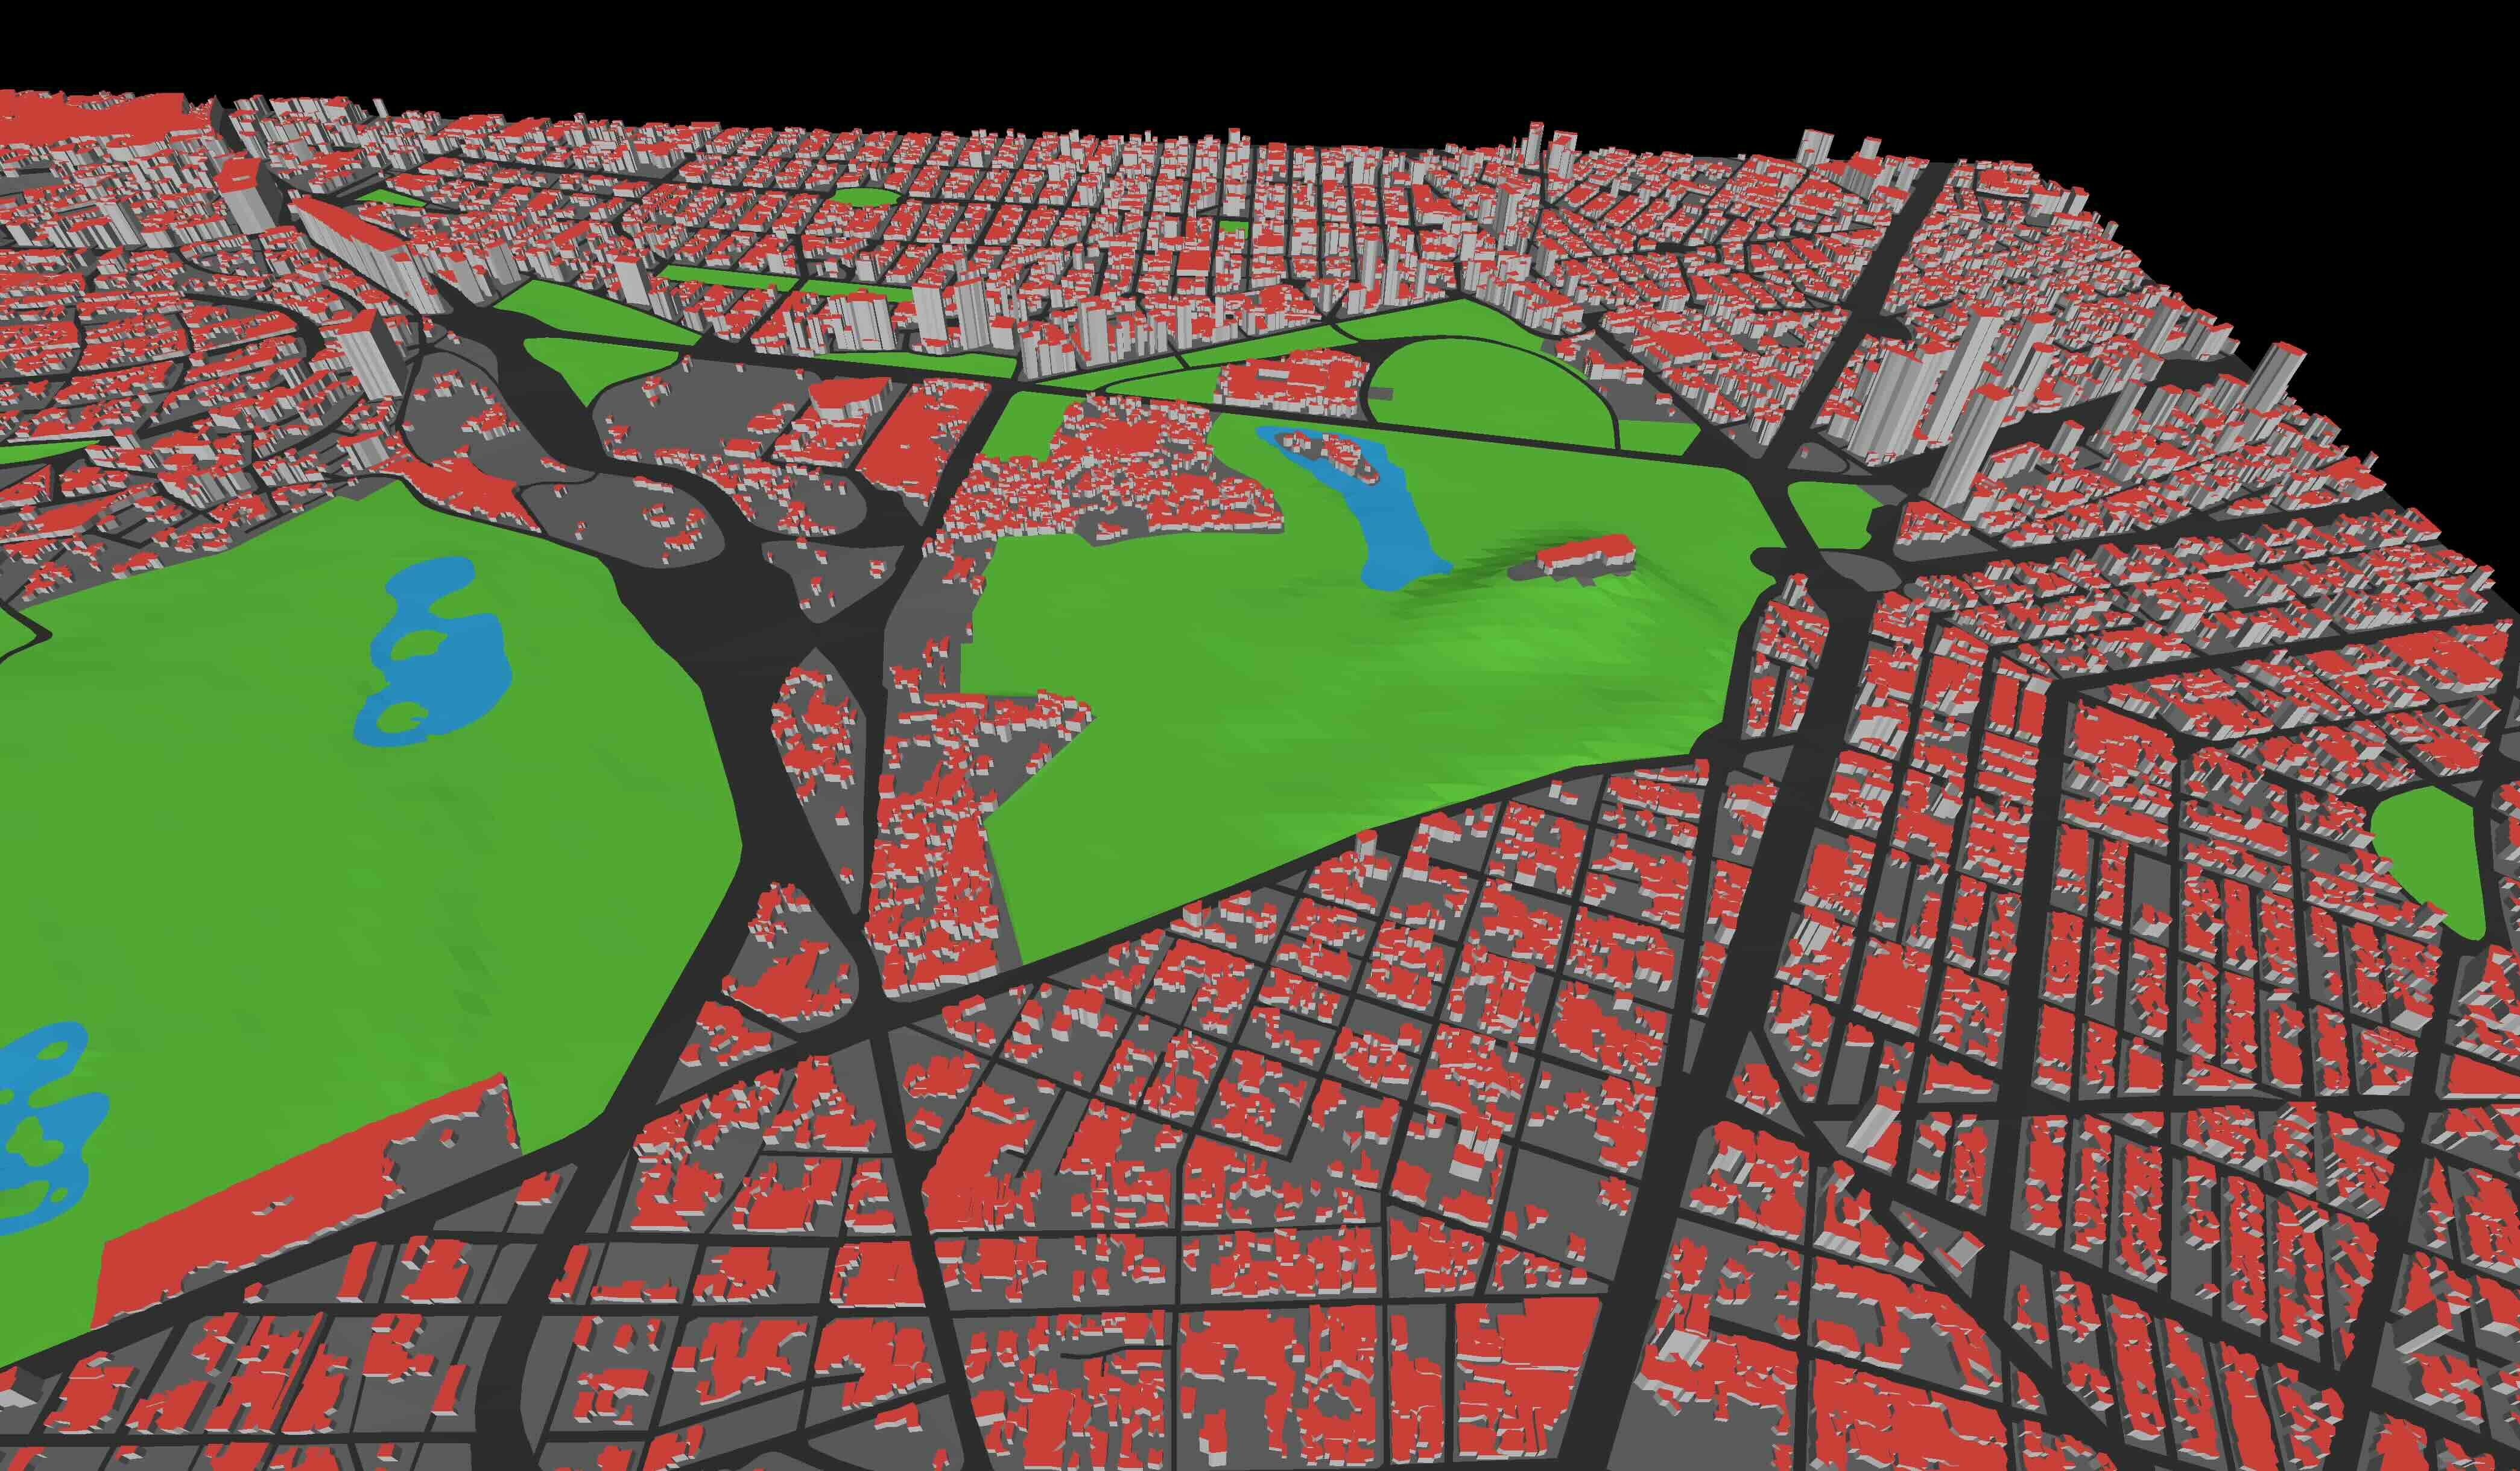
\includegraphics[width=\linewidth]{figures/snapshot01.jpg}
    \caption{}
    \label{fig:snapshot01}
\end{subfigure}
\begin{subfigure}{\linewidth}
    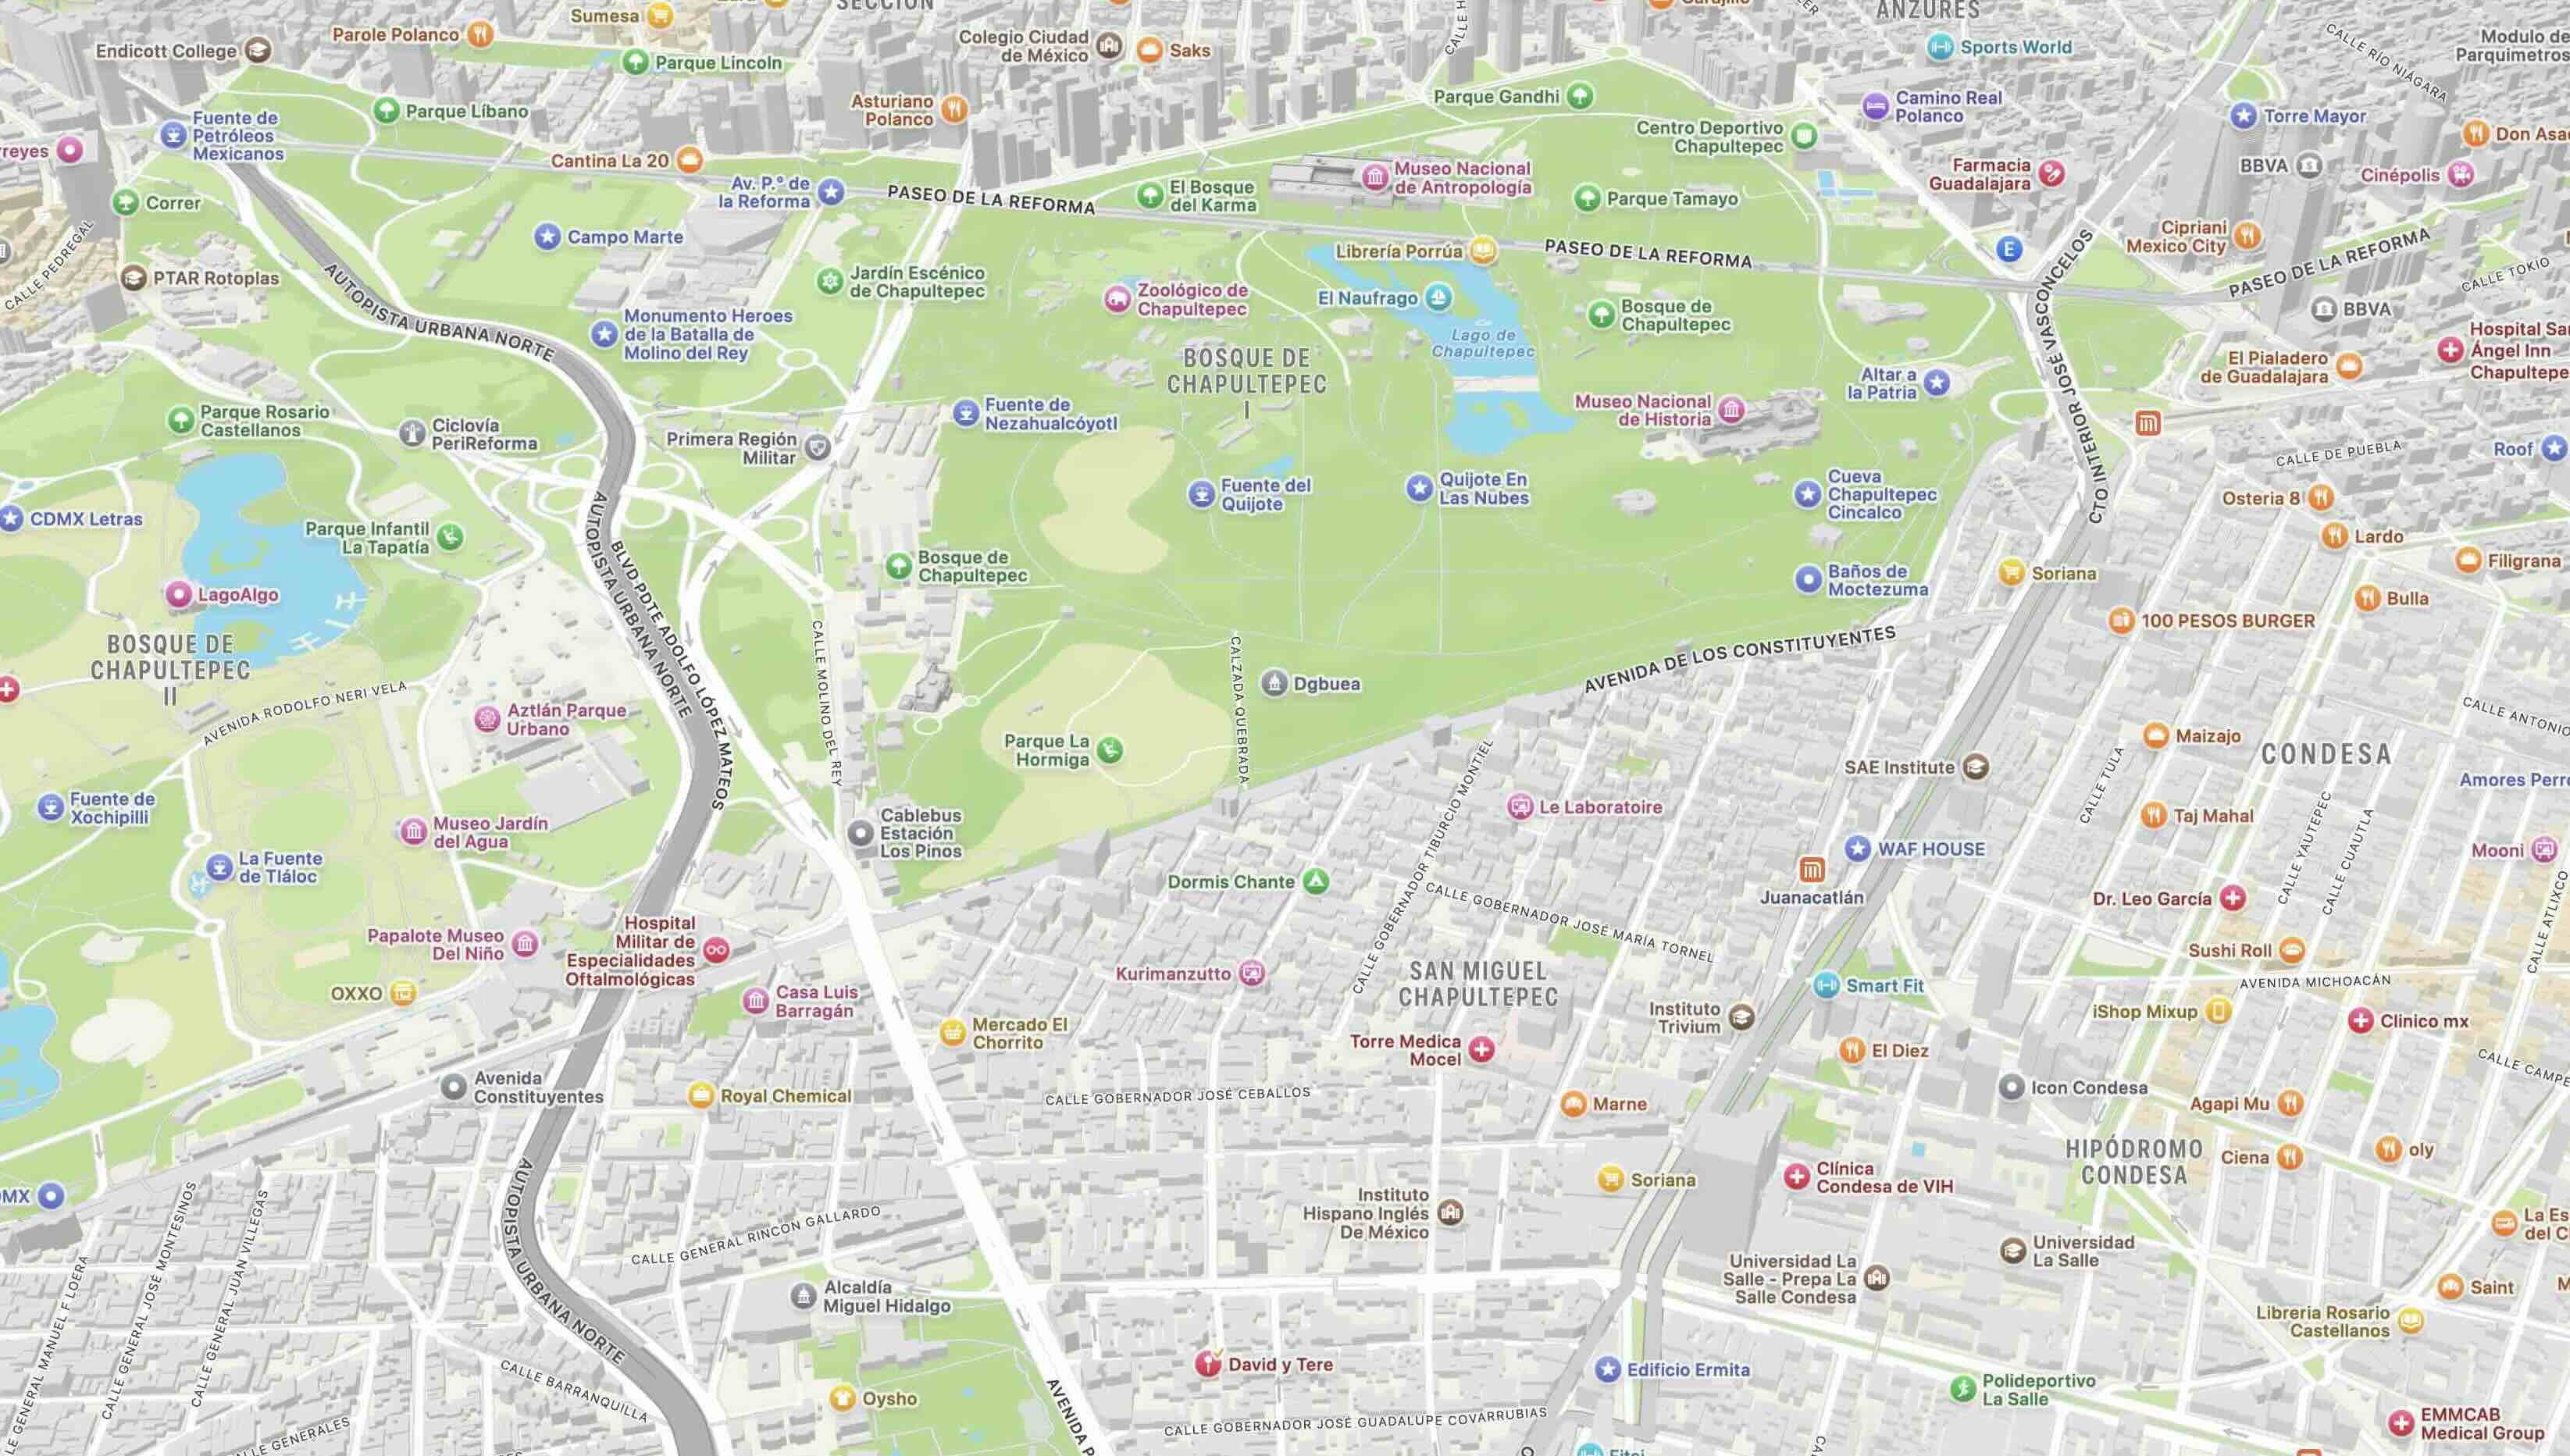
\includegraphics[width=\linewidth]{figures/apple.jpg}
    \caption{}
    \label{fig:apple}
\end{subfigure}
\caption{(a) A view of the 3D city model created using our methodology and (b) a similar view using the recently released detailed map data in Apple Maps for comparison. Note the similarities in the most distinctive buildings and the road areas. Apple Maps does not use relief within the map, even in the 3D view.}
\label{fig:snapshots}
\end{figure}

Lacking ground truth data that can be used for quantitative testing, we can analyse some of the qualities of the 3D city model created using the methodology presented here.
Among the positive aspects, we can highlight the following:

\begin{itemize}
    \item Most of the landmark buildings are clearly visible and recognisable. Since their heights are derived from the DSM, they are also accurate. The heights of well-known buildings also match those found online.
    \item The road polygons created are quite accurate, both in terms of their placement on the map and in terms of their width. Road hierarchies can be clearly discerned by the different road widths.
    \item The building footprints generated are also quite accurate, and outperform those available from the open building footprint datasets from Microsoft and Google in the study area. Most large buildings are captured, including non rectilinear ones, the over- and undersegmentation in these datasets is not present, and buildings on forbidden areas (e.g. roads) can be easily avoided.
\end{itemize}

Similarly, some of the negative aspects are the following:

\begin{itemize}
    \item The method is not able to generate building footprints for a significant number of buildings (roughly 30\%). These consist of smaller buildings that cannot be easily recognised in the DSM, buildings in areas that were not considered by the algorithm (e.g.\ green areas), and some buildings with uncommon architectural styles that have greater height differences between pixels than those set in the algorithm parameters.
    \item Tall ($>$10 m) uniform vegetation in areas that are not eliminated from the building footprint generation algorithm are recognised as buildings (Figure \ref{fig:snapshot02}).
    \item Terrace-shaped buildings with different parts at very different heights are recognised as different buildings (Figure \ref{fig:snapshot03}), whereas adjacent buildings of the same height are merged.
    \item 3D road structures (e.g.\ overpasses and highway interchanges) are not modelled by the method, which sets all roads at the (simplified) DTM height.
\end{itemize}

\begin{figure}[htb]
\begin{subfigure}{\linewidth}
    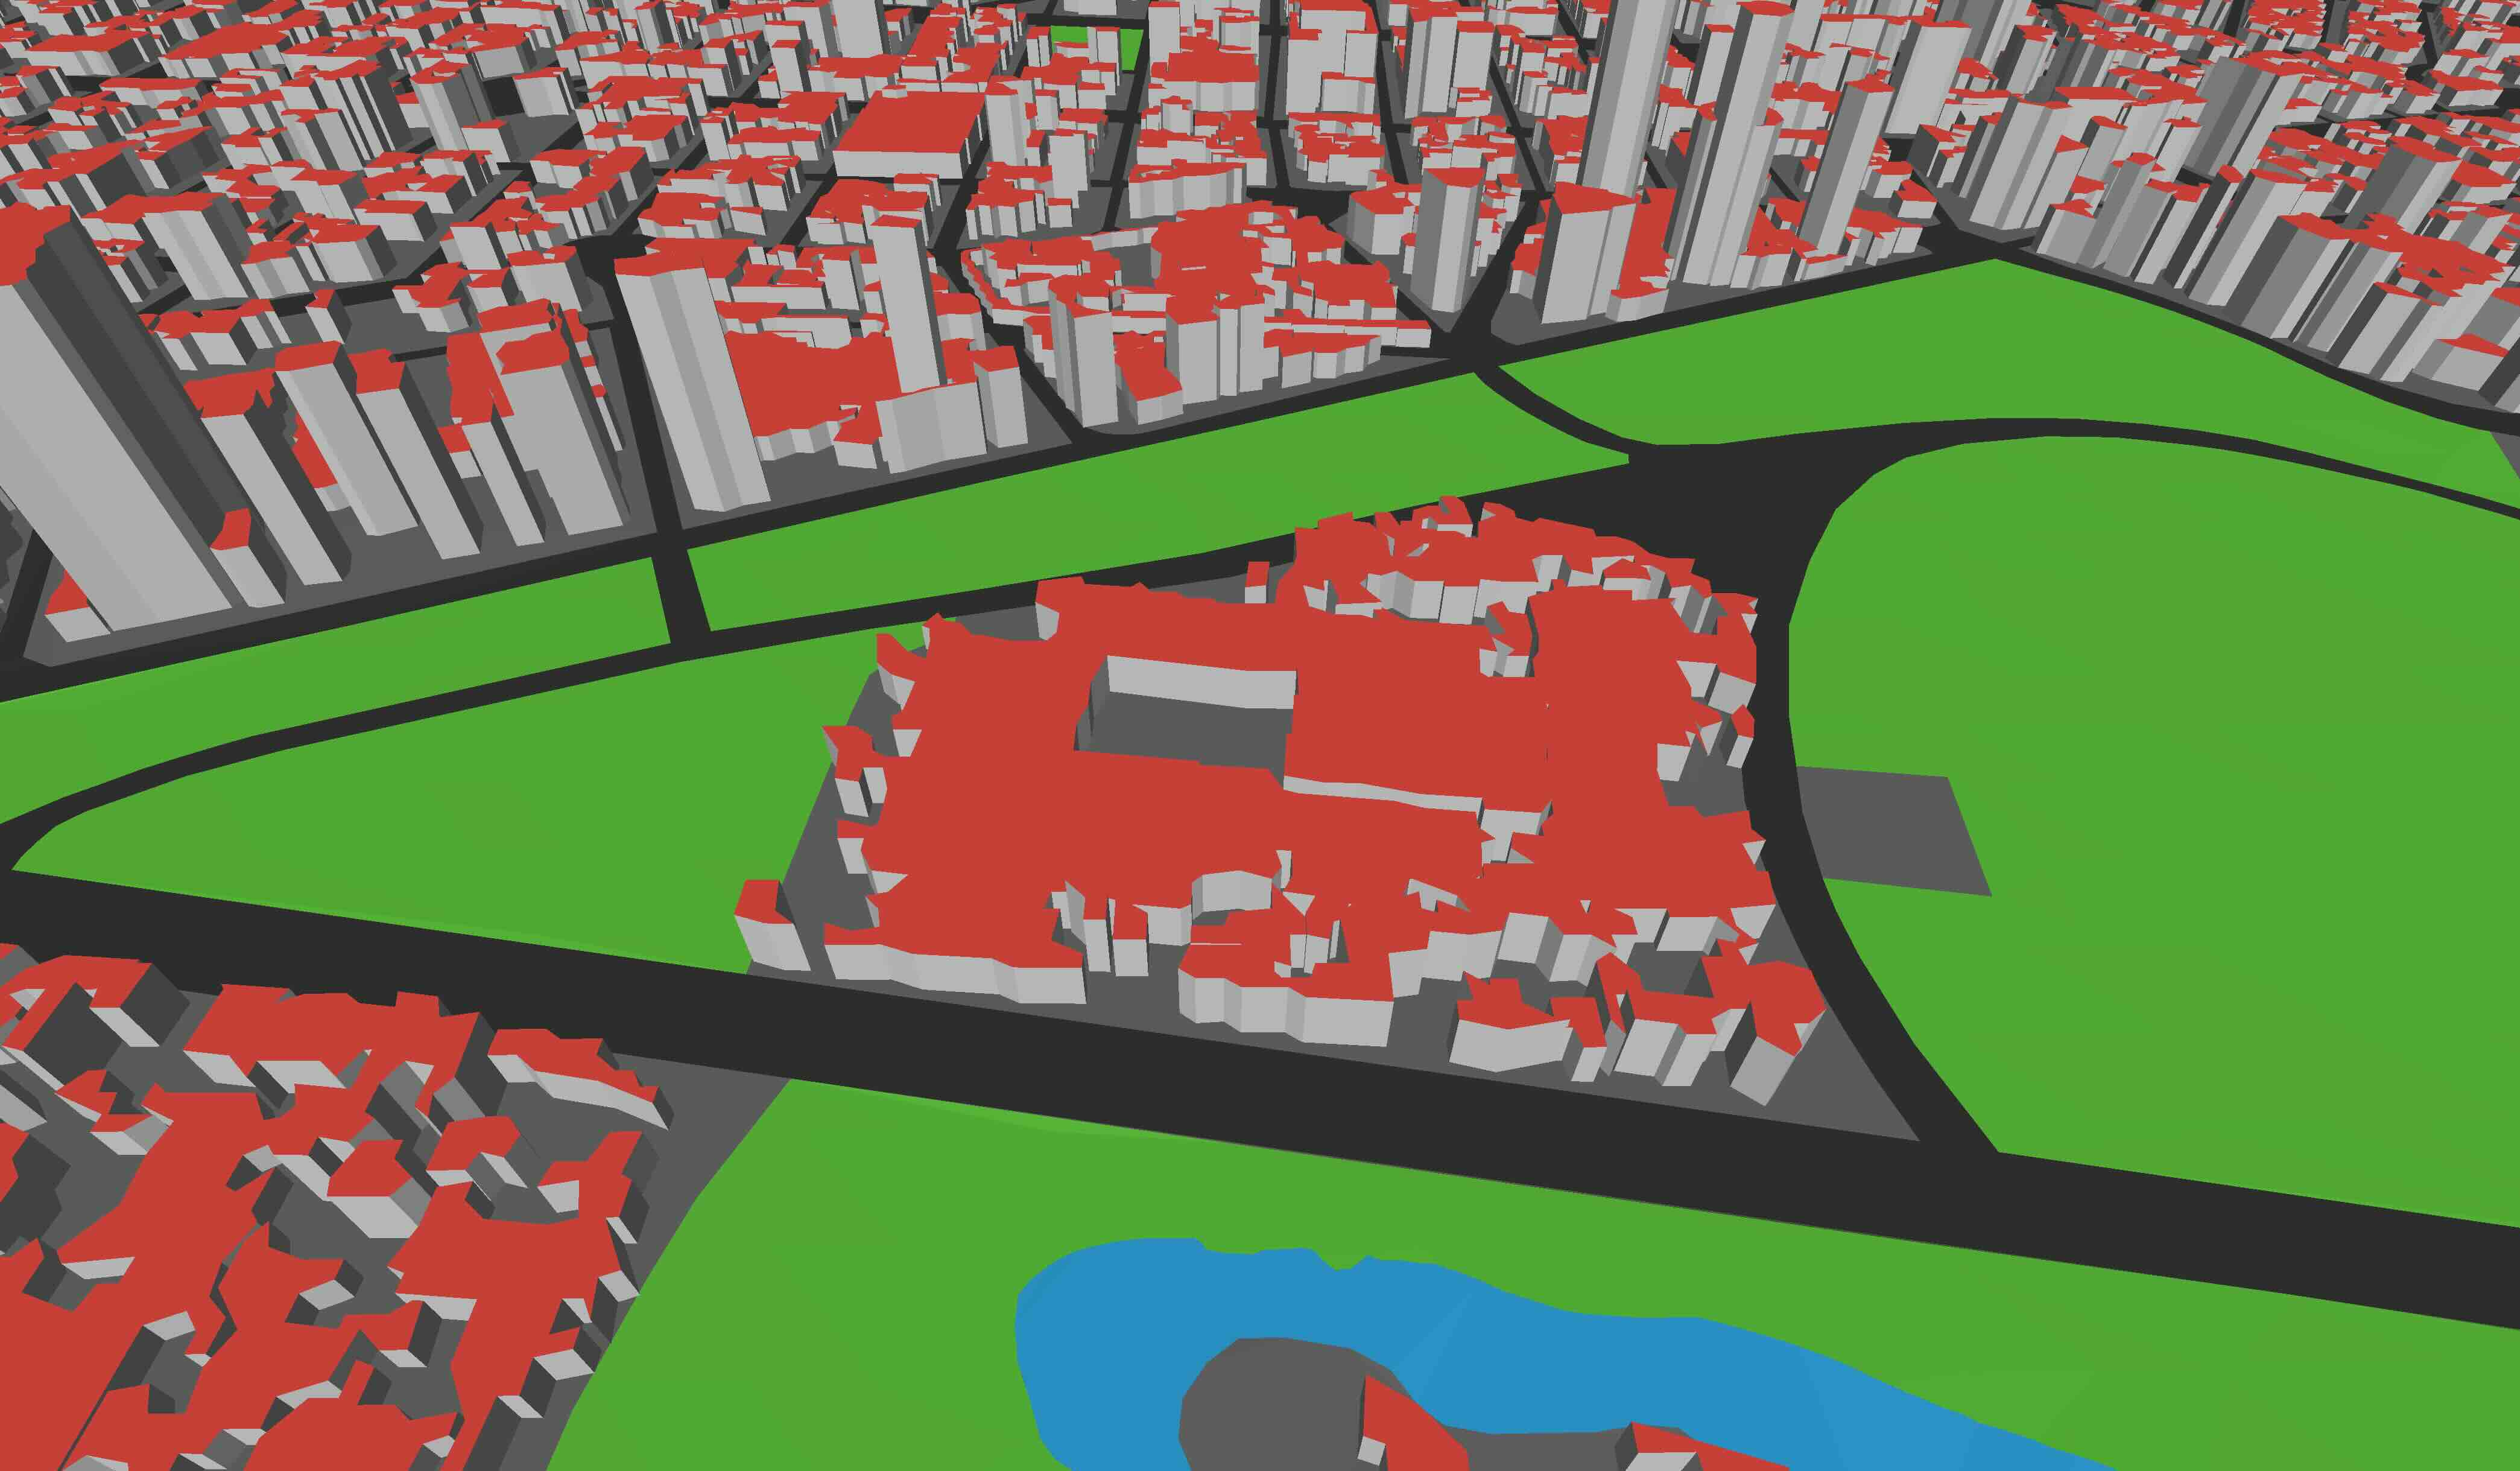
\includegraphics[width=\linewidth]{figures/snapshot02.jpg}
    \caption{}
    \label{fig:snapshot02}
\end{subfigure}
\begin{subfigure}{\linewidth}
    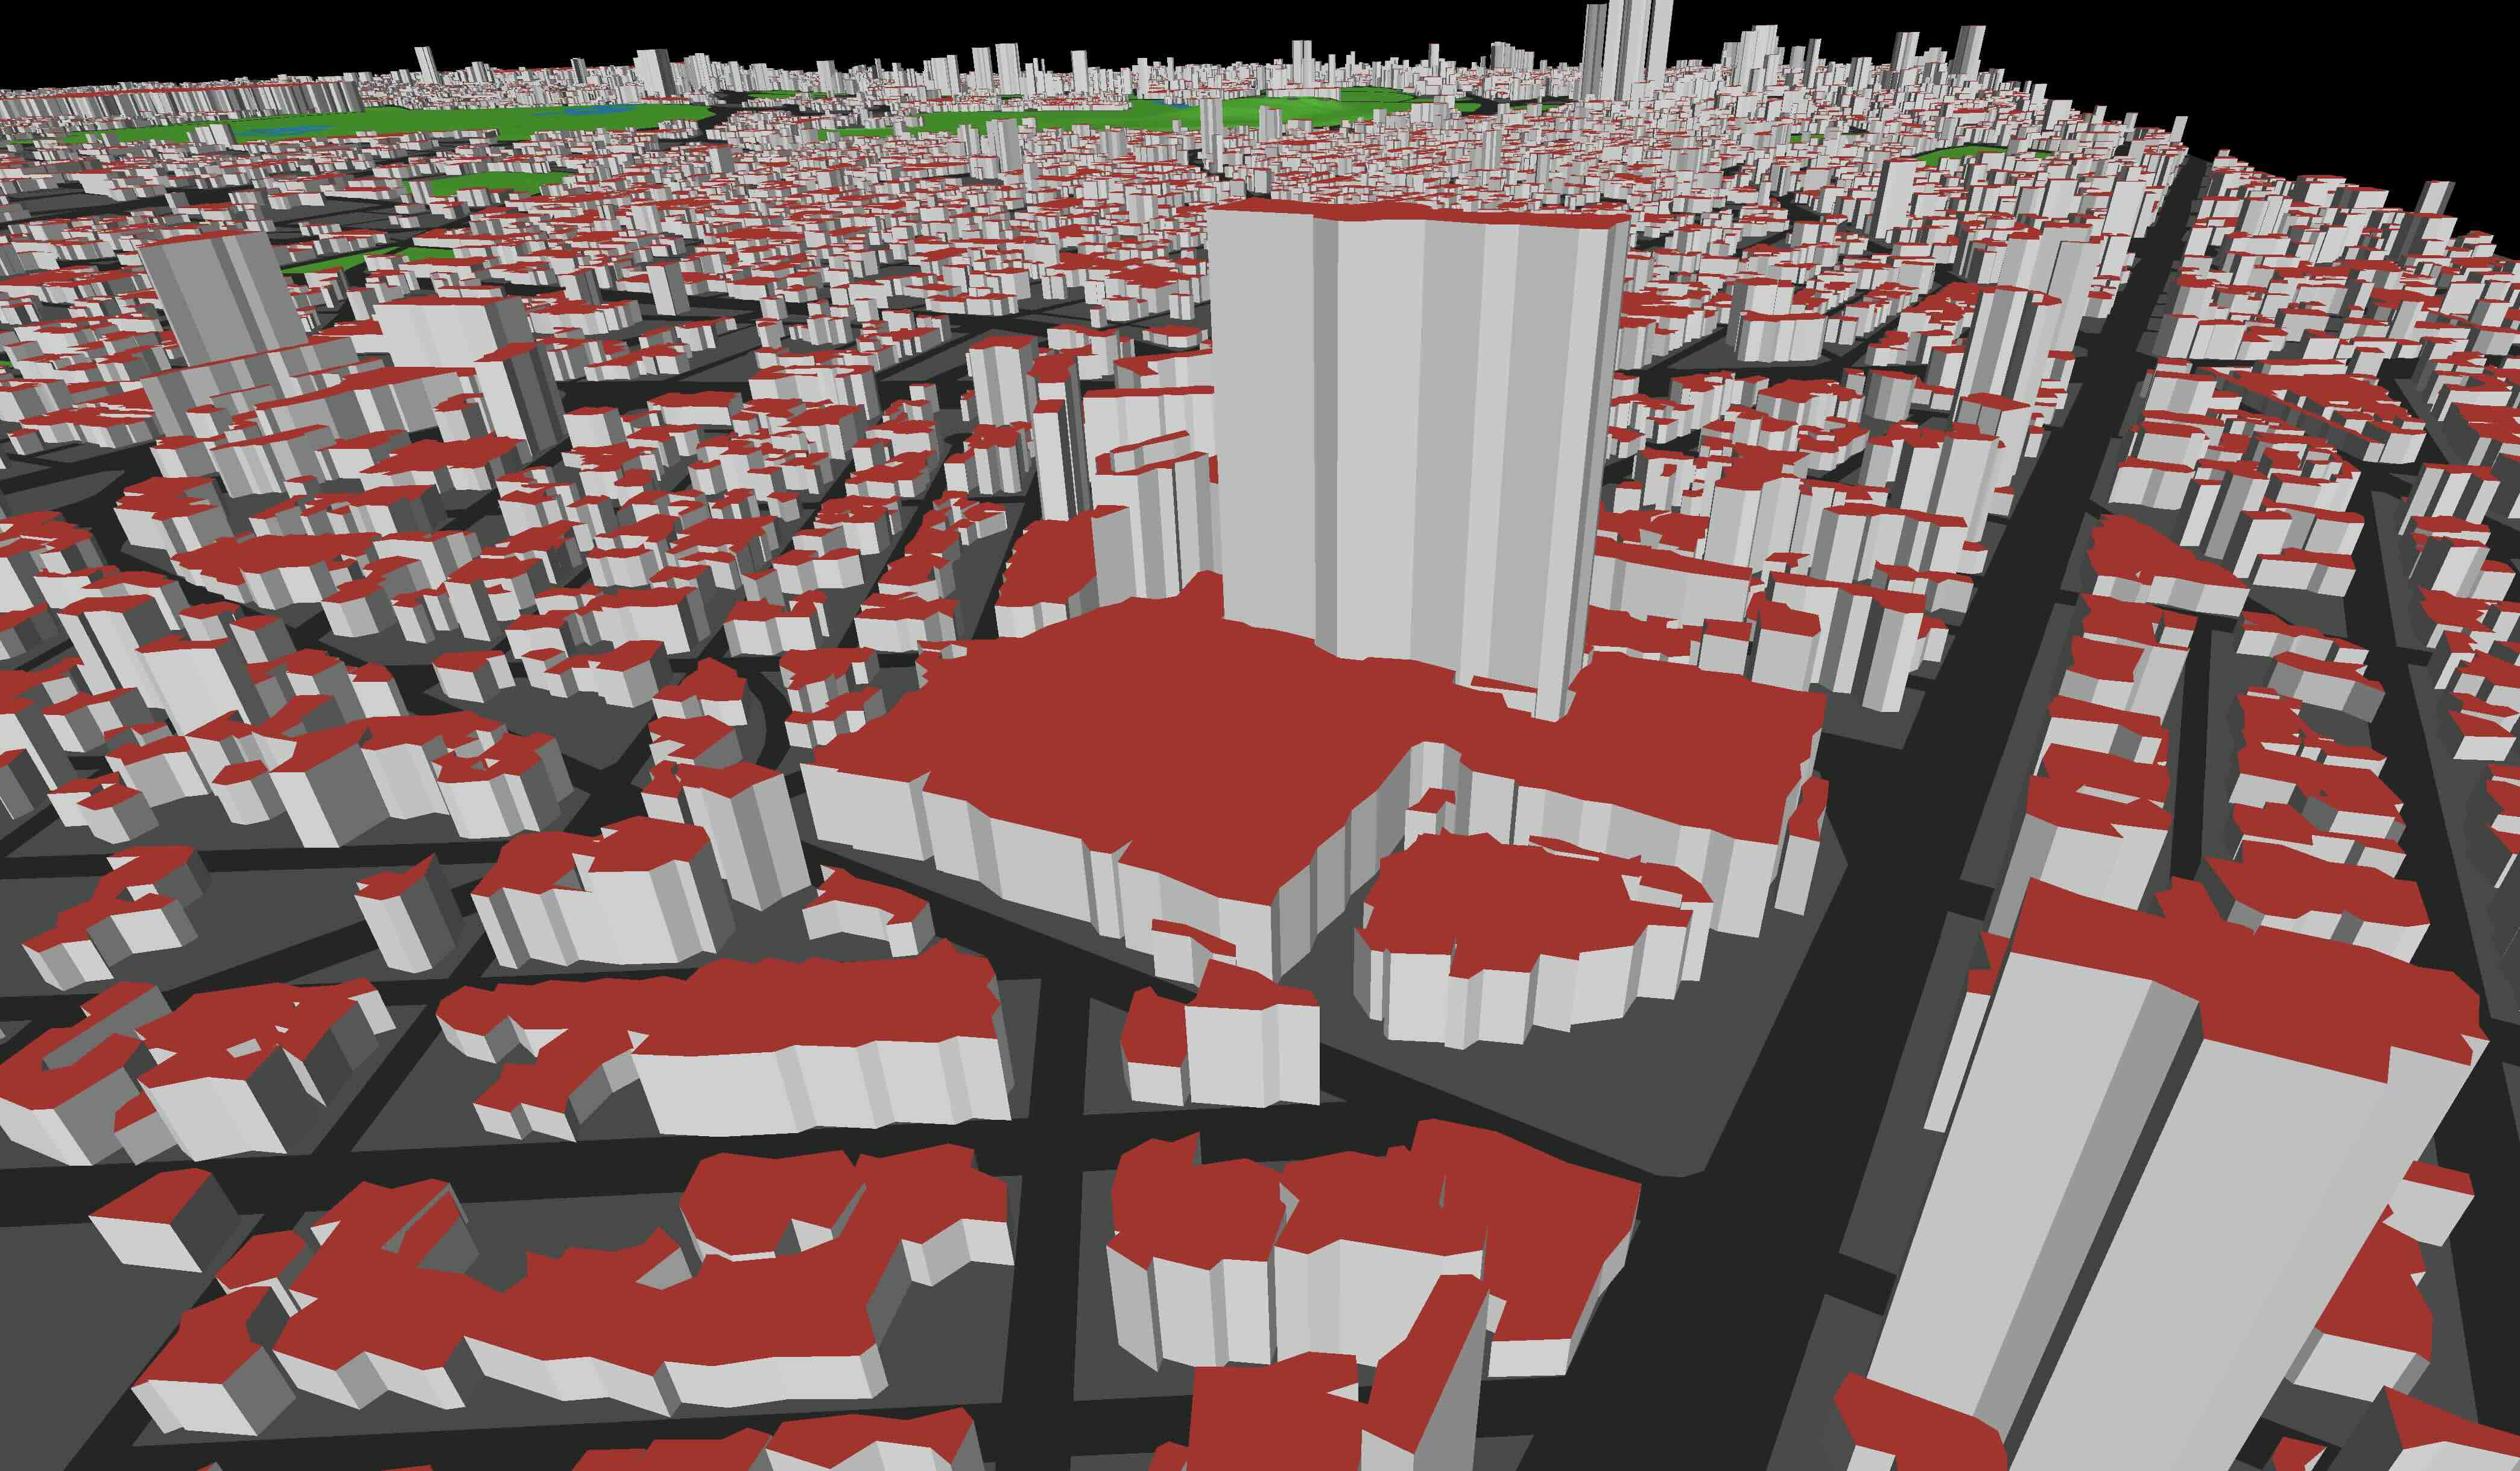
\includegraphics[width=\linewidth]{figures/snapshot03.jpg}
    \caption{}
    \label{fig:snapshot03}
\end{subfigure}
\caption{Some of the issues present in the generated 3D city model: (a) spurious buildings from vegetation around the National Museum of Anthropology and (b) the terraced architecture of the World Trade Center recognised as multiple buildings.}
\label{fig:issues}
\end{figure}

\section{Conclusions}
\label{sec:conclusions}

In this paper, we have presented a novel methodology to create 3D city models for Mexican cities using solely the open data available from INEGI.
The methodology involves several new aspects not previously tackled by other methodologies and is specifically designed around the particularities of Mexican data, including the generation of building footprints and road polygons.
While still at an early development stage, the footprint generation method is already able to outperform the building footprint datasets from Microsoft and Google for dense urban areas. 
The road polygons and building heights are also accurately derived from the source data. 

The work conducted for this paper was constrained by time limits and can be extended in different directions.
Future work can include conducting tests in other areas, fine-tuning the different generation parameters (percentiles, minimum areas and heights, maximum height differences), applying the polygon lifting algorithms differently, creating 3D road structures and using a more sophisticated DTM TIN simplification method.
In particular, using a more sophisticated algorithm to identify the buildings in the DSM data should yield significant benefits.
While the aggressive rectilinear regularisation in the Microsoft and Google datasets is not advisable, a more flexible rectilinear optimisation approach could also improve the footprint geometries.

{
	\begin{spacing}{1.17}
		\normalsize
		\bibliography{ISPRSguidelines_authors} % Include your own bibliography (*.bib), style is given in isprs.cls
	\end{spacing}
}

\end{document}
